\documentclass{article}

% Language
\usepackage[british]{babel}

% Set page size and margins
\usepackage[a4paper,top=2cm,bottom=2cm,left=3cm,right=3cm,marginparwidth=1.75cm]{geometry}

% Don't break paragraphs
\widowpenalties 1 10000
\raggedbottom

% Useful packages
\usepackage[nottoc]{tocbibind}
\usepackage{parskip}
\usepackage{array}
\usepackage{float}
\usepackage{csquotes}
\usepackage{datetime}
\usepackage{amsmath}
\usepackage{rotating}
\usepackage{graphicx}
\usepackage[dvipsnames]{xcolor}
\usepackage{listings}
\usepackage[colorlinks=true, allcolors=black]{hyperref}
\usepackage{lastpage}
\usepackage[acronym, toc]{glossaries}
\usepackage{fancyhdr}
\usepackage[UKenglish]{isodate} % UK date format
\usepackage[titletoc, toc, page]{appendix}
% Bibliography
\usepackage[backend=biber, style=numeric, sorting=none]{biblatex}
\addbibresource{bibliography.bib}

% Figures are in figures/
\graphicspath{ {figures} }

% Code style
\definecolor{backcolour}{rgb}{0.97,0.97,0.97}
% LTeX: enabled=false
\lstdefinestyle{csharp}{
    language=[Sharp]C,
    backgroundcolor=\color{backcolour},   
    commentstyle=\color{Green},
    keywordstyle=\color{blue},
    numberstyle=\small\color{teal},
    stringstyle=\color{Maroon},
    basicstyle=\ttfamily\small,
    breakatwhitespace=false,         
    breaklines=true,                 
    captionpos=b,                    
    keepspaces=true,                 
    numbers=left,                    
    numbersep=5pt,                  
    showspaces=false,                
    showstringspaces=false,
    showtabs=false,                  
    tabsize=2
}
% LTeX: enabled=true

% Header and Footer
\renewcommand{\headrulewidth}{0pt} % Header rule
\renewcommand{\footrulewidth}{0pt} % Footer rule
\pagestyle{fancy}
\fancyhf{}
\rhead{Candidate number: 1692, Centre number: 31155}
\lhead{Nathaniel Taulbut}
\lfoot{H446, 2023}
\rfoot{Page \thepage\ of \pageref{LastPage}}
% on the first page
\fancypagestyle{plain}{%
\fancyhf{}
\chead{}
\cfoot{Candidate number: 1692, Centre number: 31155}
\lfoot{H446}
\rfoot{2023}}

% Font
\usepackage{helvet}
\renewcommand{\familydefault}{\sfdefault}

% Title
\title{Air Traffic Control Simulator: OCR GCE A Computer Science Project}
\author{Nathaniel Taulbut}
\date{\today}

% Glossary
\makenoidxglossaries
\newglossaryentry{interface}{name=interface, description={An abstract type that describes attributes and methods that classes must implement}}
\newglossaryentry{airspeed}{name=airspeed, description={The speed of an aircraft relative to the air measured in knots}}
\newglossaryentry{flightpathangle}{name=flight path angle, description={The angle in degrees of an aircraft relative to the horizon, with negative values being below the horizon}}
\newglossaryentry{vector}{name=vector, description={A movement from one coordinate to another, sometimes also used as a synonym of \gls{heading}}}
\newglossaryentry{directionvector}{name=direction vector, description={A vector with a magnitude of one used to represent spatial direction}}
\newglossaryentry{instrumentapproach}{name=instrument approach, description={A predetermined path designed to guide an aircraft from near an airport to a landing}}
\newglossaryentry{heading}{name=heading, description={A compass direction in degrees}}
\newglossaryentry{waypoint}{name=waypoint, description={A point defined by latitude and longitude used for navigation}}
\newglossaryentry{airspace}{name=airspace, description={Defined three-dimensional space in the sky}}
\newglossaryentry{unitvector}{name=unit vector, description={A \gls{vector} with a magnitude of one}}
\newglossaryentry{quadrant}{name=quadrant, description={One of four infinite regions of a two-dimensional Cartesian system created by dividing the plane by the axes}}
% Acronyms
\newacronym{vfr}{VFR}{visual flight rules}
\newacronym{ifr}{IFR}{instrument flight rules}
\newacronym{ils}{ILS}{Instrument landing system}
\newacronym{atc}{ATC}{Air Traffic Control}
\newacronym{atco}{ATCO}{Air Traffic Controller}
\newacronym{nats}{NATS}{National Air Traffic Services}
\newacronym{vatsim}{VATSIM}{Virtual Air Traffic Simulation Network}

% ------------ Document ------------
\begin{document}

% ------- Cover page -------
\begin{titlepage}
    \maketitle
    % \begin{abstract}
    % \end{abstract}
    %\begin{center}
    %An OCR GCE A Computer Science Project
    %\end{center}
    \vspace{70pt}
    \noindent\makebox[\textwidth]{\includegraphics[width=\paperwidth]{pictures/heathrow_night_1.jpg}}
    % \includegraphics[width=\textwidth]{heathrow_night_1.jpg}
\end{titlepage}

% Blank page for cover
\shipout\null

% Table of contents
\tableofcontents
\clearpage

% List of figures and listings
\listoffigures
\addcontentsline{toc}{section}{List of Listings}
\lstlistoflistings

\vfill
\begin{center}
Typeset in \textrm{\LaTeX{}}
\end{center}

\clearpage

\section{Introduction}
\begin{figure}[H]
\centering
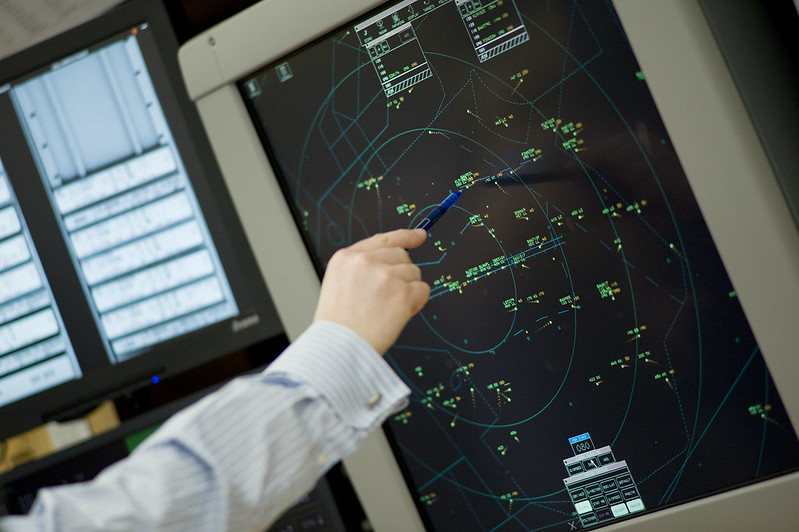
\includegraphics[width=0.85\textwidth]{pictures/nats_radar.jpg}
\caption{\label{fig:radar}A radar display at Swanwick \acrshort{atc} centre (\href{https://www.nats.aero/}{NATS}, \href{https://creativecommons.org/licenses/by-nc-nd/2.0/}{CC BY-NC-ND 2.0})}
\end{figure}

My project is an air traffic control simulator.
\acrfull{atc} is a service provided by air traffic controllers, who issue instructions and provide information to aircraft on the ground and in the air.
Air traffic controllers monitor the position of aircraft using radar, as shown in Figure \ref{fig:radar}, and communicate with pilots using radio\cite{caadef}.


\section{Analysis}
\subsection{Problem identification}
There are three main types of air traffic controllers: Aerodrome, Area, and Approach.

Aerodrome Controllers issue clearances to take off and land and route aircraft around the airfield; Area Controllers are responsible for aircraft in the climb, descent and en-route phases of flight; and Approach Controllers manage aircraft approaching an airport, putting them into the most efficient sequence to land\cite{natscareers}.

An air traffic controller is responsible for a particular section of \gls{airspace}.
Aircraft will arrive into their area of responsibility from certain points, and they will have to guide the traffic to the next controller's area of responsibility.
For example, a plane enters an approach control area descending from cruise, and the controller must guide them to an approach for a certain runway, where they are transferred to the aerodrome controller.

There are existing solutions for real-world training of air traffic controllers, and for public use.
Because the solutions for real-world controllers require certification, my solution will focus on public use.
My solution will aim to improve on the areas that are lacking in the existing publicly available solutions.

This problem is amenable to a computational approach because there is no other way to create this kind of simulation.
Real-world air traffic control relies heavily on computers.
This and the use of computational methods will be expanded on in the feature subsections of section \ref{essentialfeatures}.

\subsection{Stakeholders}
The two primary stakeholders for my solution are hobbyists and air traffic control organizations.
Their needs both include realism and ease of use.
The design section (\ref{design}) will discuss how decisions have been made to meet these needs.

\subsubsection{Air Traffic Control organizations}
The UK's \acrfull{nats} organization has a basic air traffic control game on their website for people to test their skills and determine if becoming an air traffic controller is right for them.
My solution could better solve that problem by providing a more realistic simulation, creating a more accurate test.
Other ATC organizations could promote the solution and make use of it to get people interested in air traffic control, making them more likely to take it up as a career, which is necessary as some \acrshort{atc} organizations struggle to recruit enough controllers\cite{indiaatcshortage}.

\subsubsection{Hobbyists}
Providing air traffic control is challenging and high-pressure.
It involves reacting to novel situations; thinking and planning ahead; and executing to move aeroplanes as safely and quickly as possible\cite{natsbuzz}.
For this reason, many people find it enjoyable to play the role of \acrshort{atc} in a simulator -- the \acrfull{vatsim}\footnote{\url{https://vatsim.net}} has over 100,000 active members as of 2023.
These users likely have an interest in air traffic control generally or want to become a controller in real life.
They will make use of the solution for entertainment as well as personal training in skills such as multitasking and problem-solving.
Because of their interests, they are likely to own a desktop or laptop computer.

Representing this group is Freddy.
He is a sixth form student who is interested in and knowledgeable about Air Traffic Control, wanting to become an RAF Air Traffic Controller in the future.
He has used multiple air traffic control simulators including Tower3D Pro and Endless ATC.
He can therefore provide very useful feedback on my solution.


\subsection{Existing solutions} \label{existingsolutions}
\subsubsection{ATC-SIM} \label{atc-sim}
\begin{figure}[H]
\centering
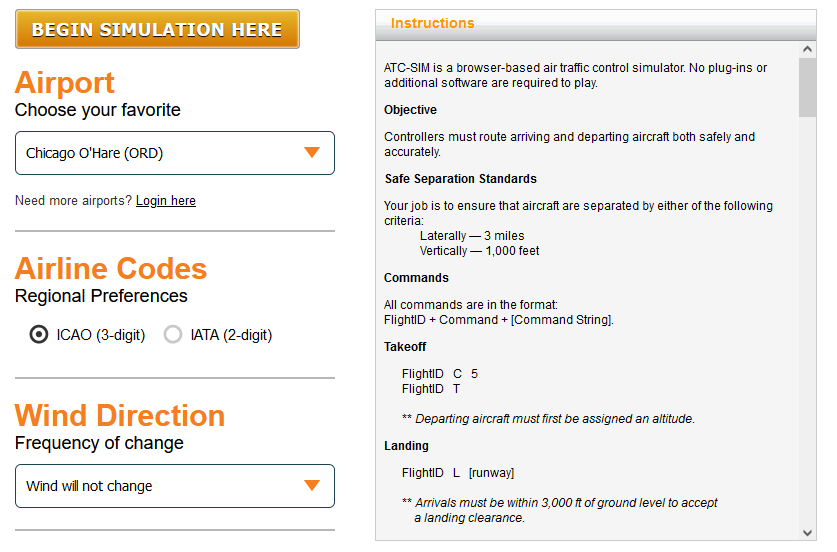
\includegraphics[width=0.7\textwidth]{existing_solutions/atcsimmenu.png}
\caption{\label{fig:atcsimmenu}ATC-SIM Main Menu}
\end{figure}
ATC-SIM\footnote{\url{https://atc-sim.com/}} is a browser-based air traffic control simulator which focuses on approach and tower control.
On the menu screen shown in Figure \ref{fig:atcsimmenu}, the user can select which airport they would like to control at and other preferences such as how much the wind will change.
It also shows instructions for the main part of the game.
The user can then press 'begin simulation here' to start, which takes them to the gameplay screen.
This serves its purpose well.
\begin{figure}[H]
\centering
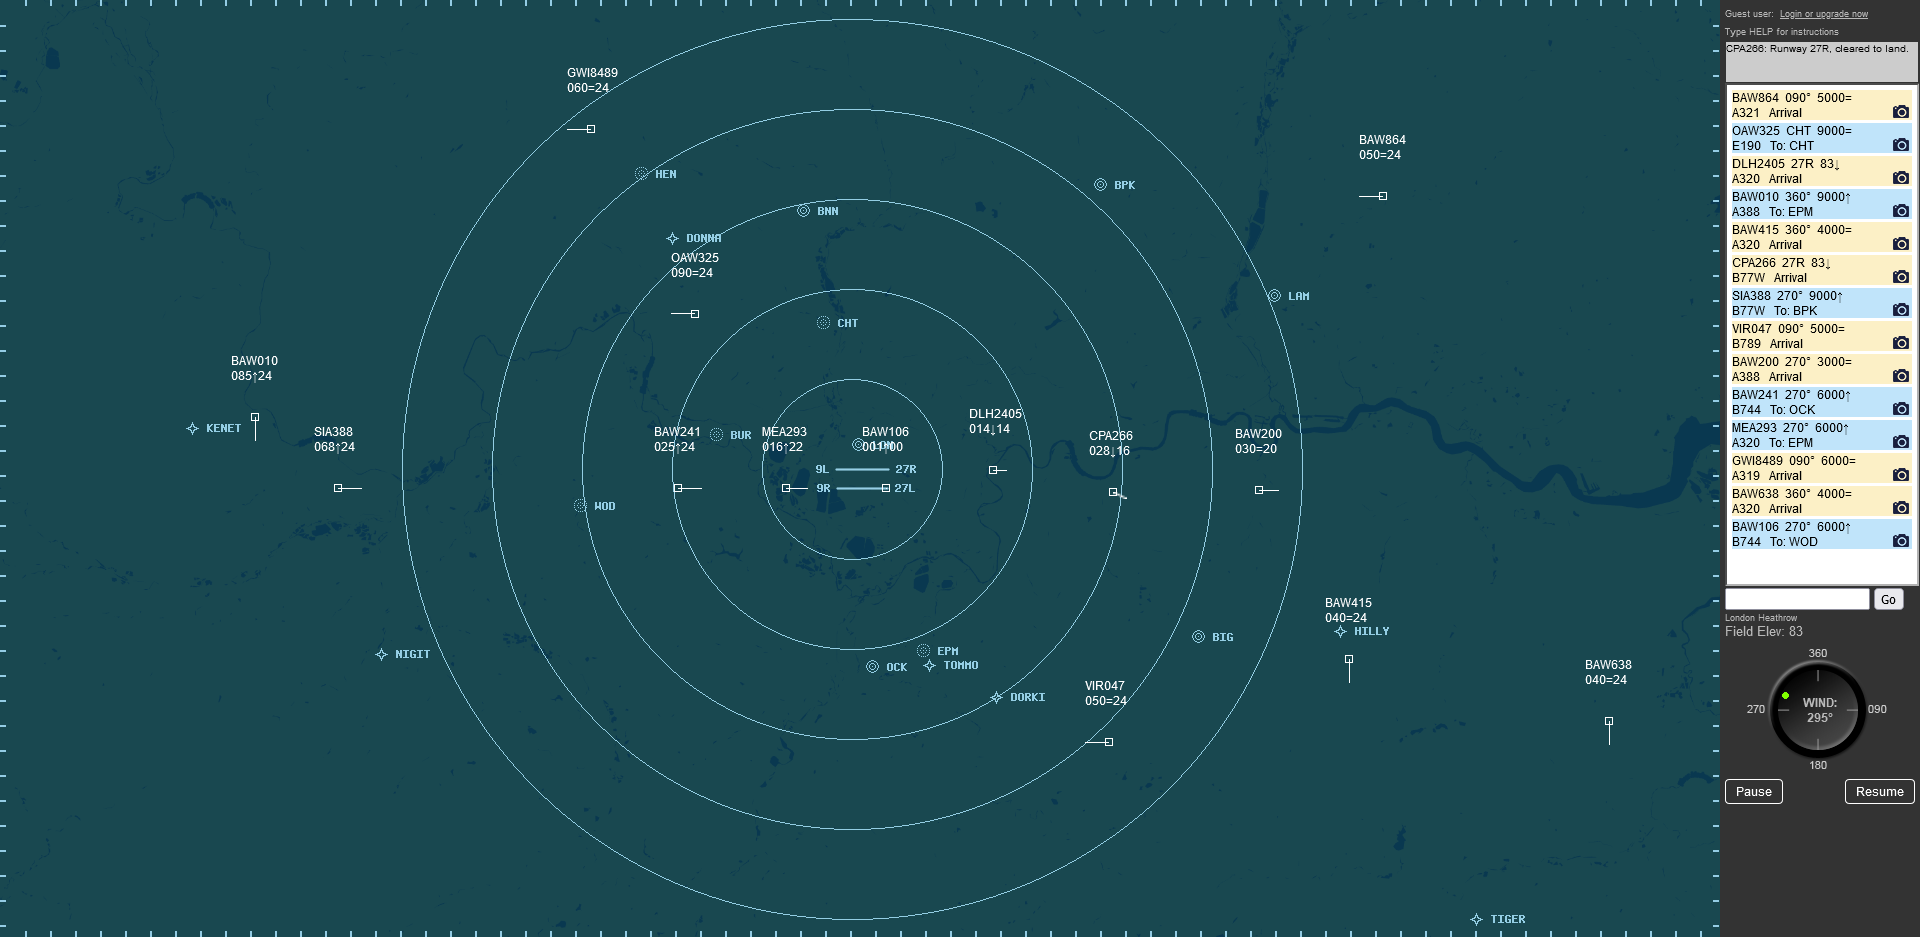
\includegraphics[width=0.85\textwidth]{existing_solutions/atcsim1.png}
\caption{\label{fig:atcsim1}ATC-SIM Gameplay Screen}
\end{figure}
The user can issue instructions to aeroplanes by entering abbreviated text commands into a text box, e.g. "BAW123 C 5" is an instruction for that aeroplane ("BAW123") to climb or descend to 5,000ft.
As seen in Figure \ref{fig:atcsim1}, a list of aeroplanes under the user's control is on the right-hand side of the screen.
On the central screen, text next to each aeroplane displays their current altitude, heading, and speed.
A display on the right-hand side shows the current wind speed and direction.
A background image shows the terrain and areas of water.

The view cannot be panned or zoomed and if the size of the browser window changes, the background moves but the waypoints don't, resulting in a visual mismatch (see Figure \ref{fig:airportinseaatcsim}).
Only a limited number of waypoints are available for the user to direct the aeroplane to.
There is no visual indication of the approach path, which makes it impossible for the user to accurately guide aeroplanes in.
Overall this is a reasonable solution for some but will disappoint more knowledgeable users.

\subsubsection{Endless ATC} \label{endlessatc}
\begin{figure}[H]
\centering
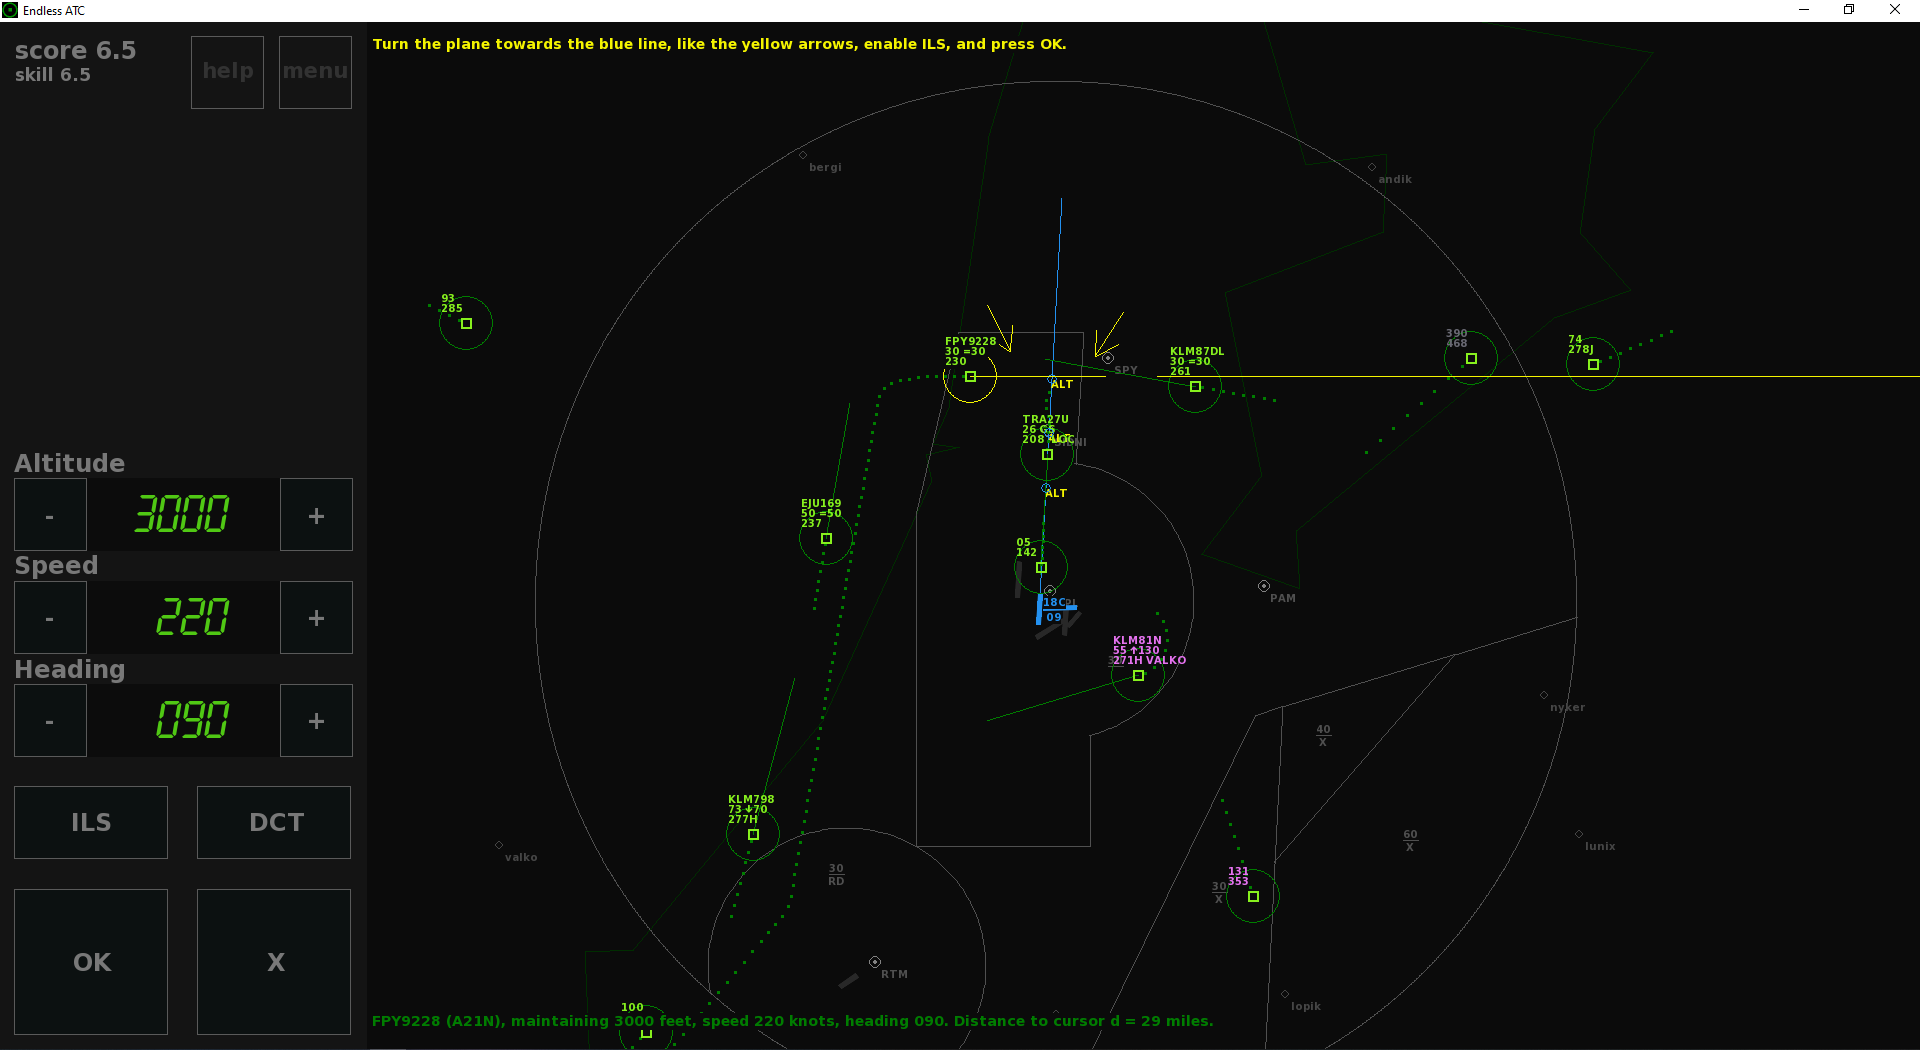
\includegraphics[width=0.85\textwidth]{existing_solutions/endlessatc.png}
\caption{\label{fig:endlessatc1}Endless ATC}
\end{figure}
Endless ATC\footnote{\url{https://startgrid.itch.io/endlessatc}} is a desktop and mobile air traffic control simulator focused on approach control.
The user can issue headings to aeroplanes by clicking or tapping on them and then moving their cursor in the direction of the desired heading.
The view can be panned around with the mouse and zoomed in with the scroll wheel.
Buttons on the side allow the user to change altitude, speed, and heading, or they can use various keys such as the scroll wheel to quickly change these values.

Once values have been changed, a button must be pressed to confirm or cancel the instructions.
A problem is that an instruction is also confirmed when the user clicks away or onto another aeroplane, potentially leading to confirming an instruction the user didn't mean to.
Text next to each aeroplane displays their current altitude, heading, and speed.
A limited number of waypoints are available which aeroplane can be directed to by clicking and dragging to them.
The coastline is shown with overly simple lines.
A limited number of customization options are available, such as changing the aeroplane icons.
Another issue is that the user can only give altitude instructions in increments of thousands of feet, whereas it is very common in reality for controllers to give instructions involving hundreds of feet.


\subsection{Features} \label{essentialfeatures}
\subsubsection{Simulated aeroplanes}
The aim of my solution is to simulate the role of an air traffic controller, and the user will therefore need some traffic to control.
Whilst some solutions require other people to 'fly' the aeroplanes, mine should allow someone to use the simulation without any additional people, making it more flexible.
To achieve this the air traffic will have to be simulated by a computer.
This will involve repeatedly calculating the aeroplane's movement many times a second based on their speed and direction, and other factors such as wind.
This can be achieved with an algorithm and mathematical calculations which are suited to being run on a computer, allowing many aeroplanes to be simulated concurrently.

These aeroplanes will be abstracted from reality, only simulating the variables that are necessary to appear realistic on a radar screen.
For example, lift does not have to be simulated --- instead it can just be stated that the aeroplane is at a particular altitude.
To make them behave realistically however, it is necessary to simulate abstractions of e.g.
the pitch of the aeroplane, because this affects how long it takes for the aeroplane to change altitude.
Because the pitch required to maintain a certain \gls{flightpathangle} changes dependent on factors that would be complicated to simulate, such as lift and speed, I can instead model vertical motion only by the \gls{flightpathangle} (see figure \ref{fig:pitchfpa}), which allows for the same realistic behaviour without having to calculate the pitch.

\begin{figure}[H]
\centering
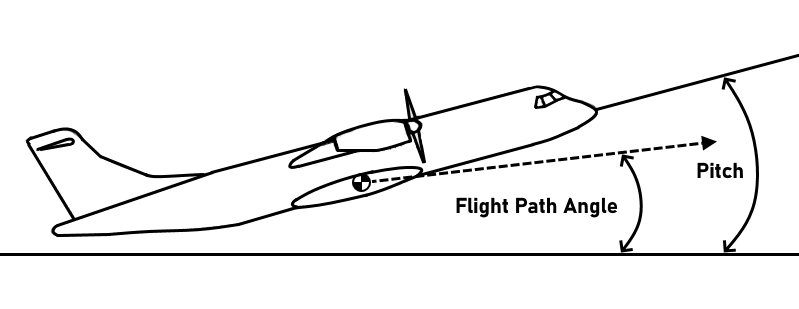
\includegraphics[width=0.7\textwidth]{diagrams/pitchfpa.png}
\caption{\label{fig:pitchfpa}Pitch and FPA}
\end{figure}

A simulation of the takeoff procedures of the aeroplane, such as its acceleration on the ground and initial rotation, will not need to be included because the solution is focussed on approach control.
Aeroplanes landing can also be largely simplified because below a certain altitude they will not be visible on the radar anyway.

Controllers often direct aeroplanes by telling them to fly on a certain heading.
The heading of an aeroplane describes the direction it is pointing in which, because of wind, is not necessarily the same as the direction it is travelling in (see Figure \ref{fig:windtriangle}).
Therefore controllers have to account for this when giving headings so that the aeroplane's actual track is in the intended direction.
This is a big part of the controller's job, so it will be necessary to simulate this.
The input to this will be a wind direction and a wind speed, live data for which could be obtained from an internet API.

\begin{figure}[H]
\centering
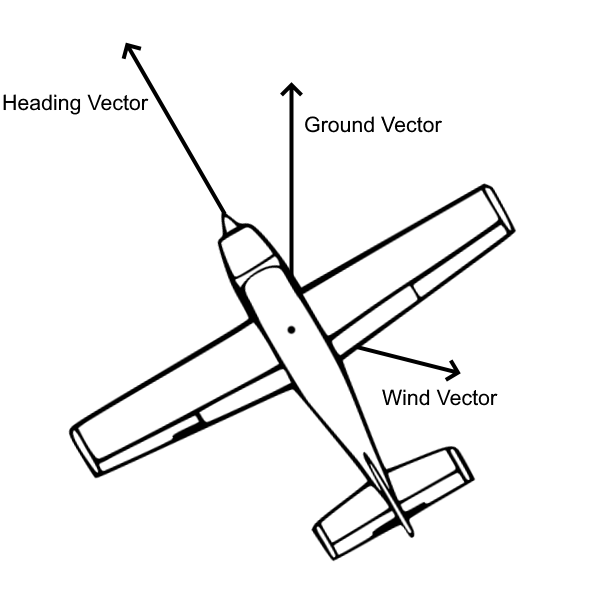
\includegraphics[width=0.5\textwidth]{diagrams/windtriangle.png}
\caption{\label{fig:windtriangle}The wind triangle}
\end{figure}

In addition to the base physics simulation, the aeroplanes will have simulated guidance systems so that they can follow the instructions defined in section \ref{aeroplaneinstructions}, one of the more complex being to follow an instrument landing system path to a landing.
An instrument landing system uses radio beacons to guide the aircraft laterally (with the localizer) and vertically (the glideslope) to a landing on the runway it is configured at, as shown in figure \ref{fig:ils}.
This can also be abstracted by not simulating the radio signals themselves.

\begin{figure}[H]
\centering
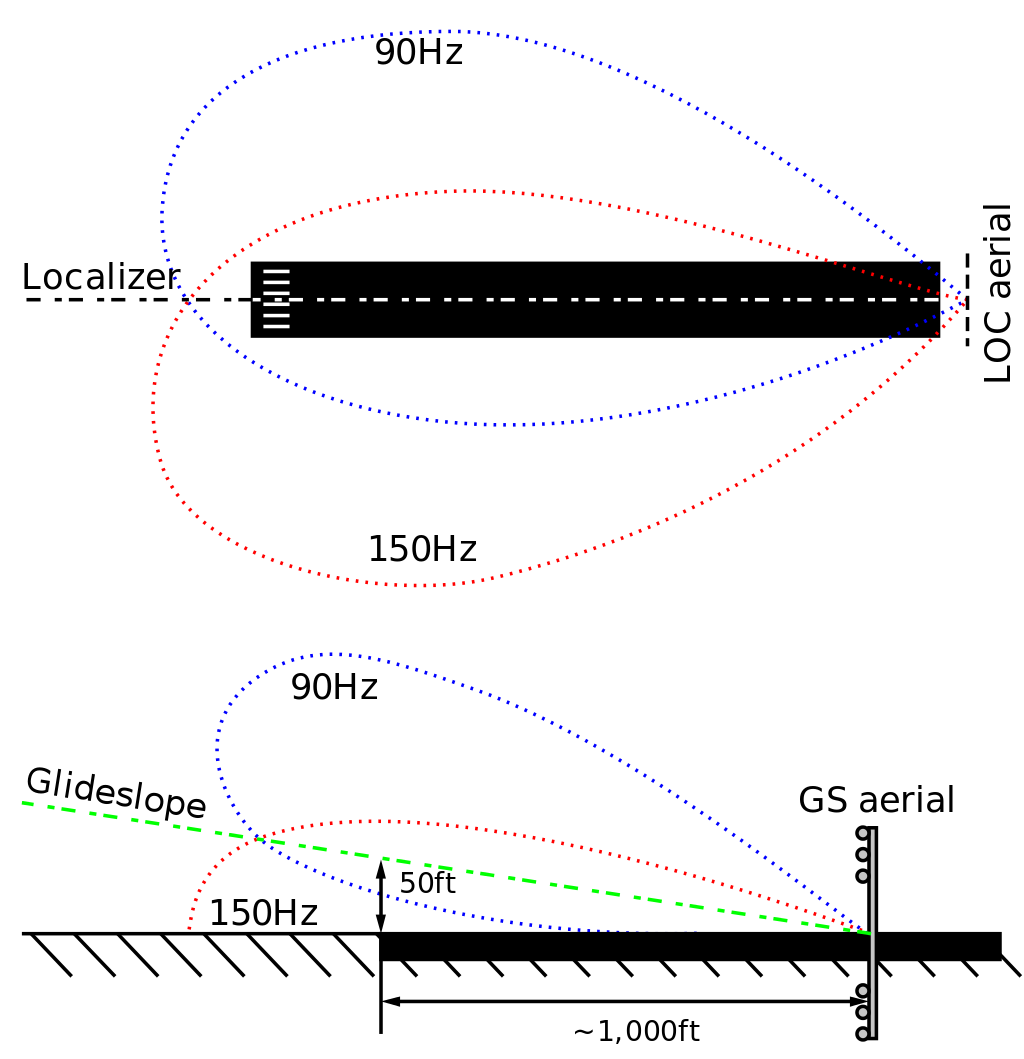
\includegraphics[width=0.5\textwidth]{context/ils.png}
\caption{\label{fig:ils}\acrfull{ils} (\href{https://commons.wikimedia.org/wiki/User:Fred_the_Oyster}{Fred the Oyster}, \href{https://creativecommons.org/licenses/by-sa/4.0/deed.en}{CC BY-SA 4.0})}
\end{figure}

\paragraph{Success criteria}
\begin{itemize}
    \item The aeroplane should be able to guide itself realistically in following instructions, including on an \acrshort{ils} (\ref{aeroplaneinstructions})
    \item The aeroplane should take a realistic amount of time to change altitude and heading
    \item Timescales should always be accurate, independent of the performance of the simulation
    \item The aeroplane's course should be accurately affected by wind
    \item Fifteen or more aeroplanes should be able to be simulated simultaneously while maintaining performance, as this is how many a controller is typically required to control in real life
\end{itemize}

\subsubsection{Aeroplane instructions} \label{aeroplaneinstructions}
In reality, air traffic controllers instruct aeroplane pilots verbally over radio.
The aeroplanes in my solution will be simulated, so there will be no pilot to hear and parse an audio instruction.
Therefore an alternative method of giving these aeroplanes instructions will be needed.
The essential instructions necessary to guide an aeroplane to a landing are for it to fly on a \gls{heading} or to a \gls{waypoint}, change altitude or \gls{airspeed}, and perform an \gls{instrumentapproach}.

The solution will create an abstraction of the verbal instructions which hides some detail, for example the user could type a number into the corresponding box and the plane will decide whether it needs to climb or descend if its current altitude is above or below the entered value.
To parse the user's input, the program will need to make multiple decisions.
For example, if the first character of the input to the heading field is an 'L' it would follow the process for instructing a turn to the left.
Also if the text was the name of a waypoint, it would send an instruction to go direct to that waypoint rather than a heading instruction.

\paragraph{Success criteria}
\begin{itemize}
    \item The user should be able to give an instruction for an aircraft to fly on a \gls{heading} or to a \gls{waypoint}, change altitude or \gls{airspeed}, and perform an \gls{instrumentapproach}; and it should respond accordingly
    \item This system should function concurrently with the simulation of the aeroplane, so that it does not pause the aeroplane's movement
    \item The solution should allow the user to give instructions as quickly or quicker than they would be able to verbally in real life
    \item To make the experience more fluid, it should also require as few button presses or mouse clicks as possible
\end{itemize}

\subsubsection{Displaying aeroplanes}
A representation of the aeroplane will need to be shown.
It will need to show their assigned heading or waypoint, altitude, and speed; their current heading or targeted waypoint, altitude, and speed; and their callsign.
As with real life radar displays, it should show a trail of dots or other symbols behind the aeroplane to illustrate its path and a line in front to show its current direction of travel.
It should be visually similar to real life for additional realism, including mimicking how quickly the display properties update, e.g. the radar only completes a full sweep every 4 seconds.
This can only be accomplished with a computer because of its unique ability to render custom, moving and changing graphics to display on an output device such as a monitor.

\paragraph{Success criteria}
\begin{itemize}
    \item The assigned heading or waypoint, altitude, and speed; current heading or targeted waypoint, altitude, speed, and callsign should be displayed
    \item Properties should update at a realistic rate: position every 4 seconds, and others at around every 0.5 seconds
    \item Every time the position updates, a history dot should be created up to a specified number, and they should then follow behind
\end{itemize}

\subsubsection{Traffic Simulation}
Once an aeroplane can be simulated, the creation of them must be controlled.
In the real world, the number of aeroplanes entering the controller's area of responsibility and departing changes based on airline timetables.
This data is unavailable, so an approximation can be used. Aeroplanes will enter and exit the controller's area of responsibility via certain waypoints.

\paragraph{Success criteria}
\begin{itemize}
    \item Aeroplanes should enter the user's area of responsibility periodically from certain waypoints
    \item Aeroplanes should appear on the screen after taking off from a runway periodically
\end{itemize}

\subsubsection{Waypoints}
\begin{figure}[H]
\centering
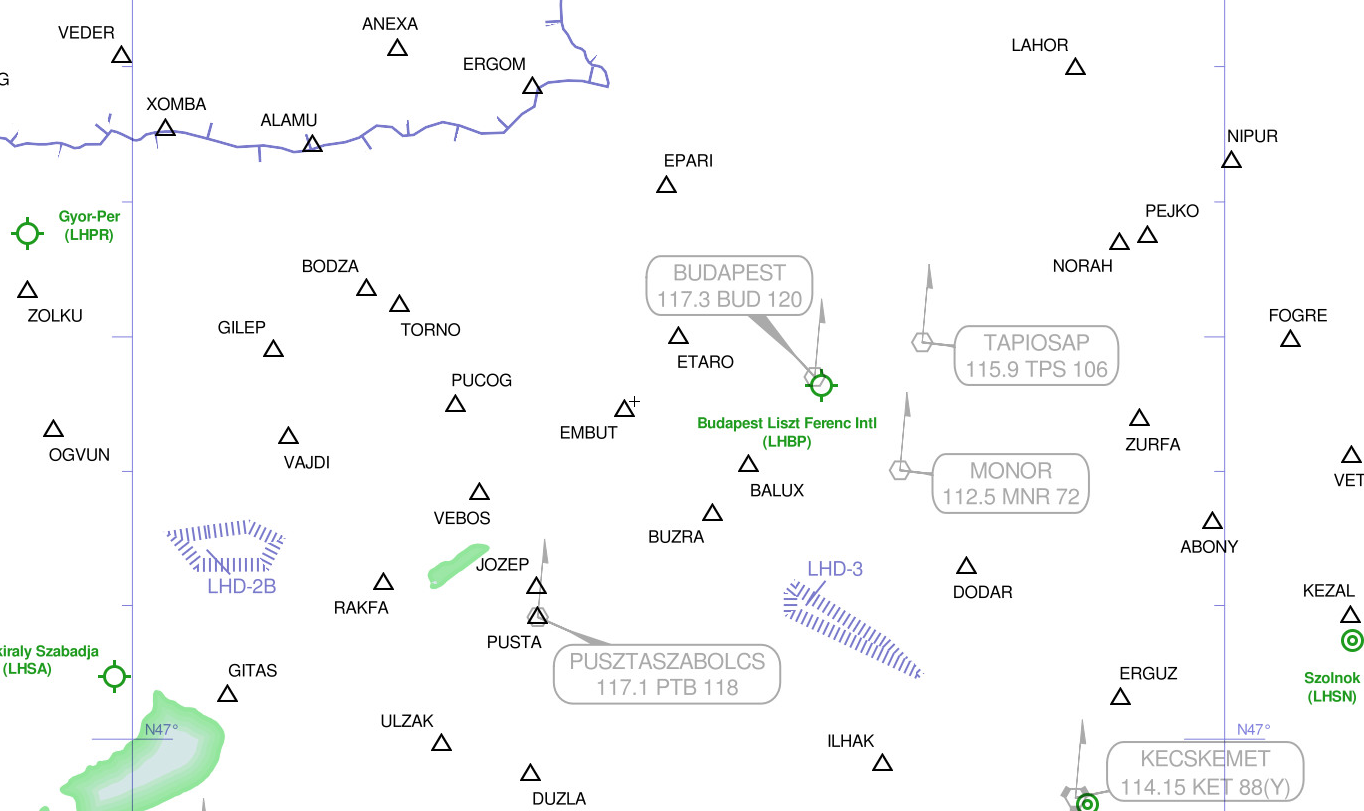
\includegraphics[width=0.7\textwidth]{context/budapest.png}
\caption{\label{fig:budapest}Map showing waypoints around Budapest International Airport}
\end{figure}

Waypoints are points, defined by latitude and longitude and given five-letter names, which are used for air navigation.
They are created specifically for that purpose and usually have no connection to features of the real world\cite{waypoint}.
A commercial airliner's route from one airport to another --- its flight plan --- is largely defined as a series of waypoints which it will fly between.
Air traffic controllers often take advantage of waypoints to direct traffic, instructing them to 'fly direct' to a named waypoint, for example "BAW123, route direct WILLO".

Waypoints are indispensable to air traffic controllers, therefore it is necessary to include them in my solution.
This will require data to be sourced with the names and GPS coordinates of the waypoints.
The waypoints should be shown on the screen in the correct position with a symbol corresponding to their type, and their name.

\paragraph{Success criteria}
\begin{itemize}
    \item Waypoints should appear in the correct position on the screen
    \item Their name should be shown next to an icon which changes based on the type of waypoint
    \item As many as 30 or more waypoints should be able to be displayed at once, since this is how many are present around some airports
\end{itemize}

\subsubsection{Pan and Zoom}
The user should be able to pan and zoom their view of the simulated radar screen.
This way they can more clearly see important areas where the majority of traffic is concentrated, rather than being limited to a fixed view.
This is especially useful where the approach control airspace area is very large and it otherwise would not be possible to simulate because there would not be enough room on the screen.
Being able to pan and zoom is also a feature of most modern real world radar screens.
To make interacting with the solution as enjoyable as possible and as professional as the real world equivalents, panning and zooming should be smooth; at a fixed speed and in fixed steps; and the camera should zoom towards the centre of the screen.
This will also create a familiar experience which is intuitive.

\paragraph{Success criteria}
\begin{itemize}
    \item Panning and zooming should be smooth
    \item It should occur at a fixed speed and in fixed steps
    \item The camera should zoom towards the centre of the screen
\end{itemize}

\subsubsection{Geographical features}
To make the simulated radar screen look realistic, it should be able to draw some kind of representation of the terrain.
Like in Endless ATC (\ref{endlessatc}), this can be a line showing the local coastline.
This is important because controllers should know if an aircraft is over water.
A large amount of data will need to be sourced representing this, which will then have to be processed and displayed.
This is a task very suited to being run a computer because of the storage and intensive processing of data.
This data will ultimately be represented using many latitude and longitude points, and looping will be necessary to apply processing to all of them.

\paragraph{Success criteria}
\begin{itemize}
    \item An abstraction of the terrain should be displayed
    \item It should appear accurate, having the correct proportions and with no breaks in lines
    \item It should respect the current scale of the display
\end{itemize}

\subsubsection{Extended centrelines}
For every instrument approach (\acrshort{ils}) available at the airport the user is controlling at, a line extending from the threshold of the relevant runway in the direction of the localizer should be displayed and distance markers should be shown along it.
As in real life, this feature is vital for the user to be able to direct aeroplanes to the instrument approach correctly, for which they need to see exactly where it is.
The distance markers are also important so that the controller can maintain a safe separation between aeroplanes.

\paragraph{Success criteria}
\begin{itemize}
    \item The line should be in the correct position and direction
    \item Distance markings should be shown at the correct intervals
\end{itemize}


\subsection{Limitations}
A few limitations must be stated to prevent the solution from becoming overly complex and to limit the scope.
They are as follows:
\begin{itemize}
    \item The simulator will only load information such as waypoints and terrain in a small area around the airport --- it will not allow the user to pan around the whole world at once.
    Doing so would require streaming the data in as the user moved around, which would be unnecessarily complex to implement because the user is only controlling aeroplanes in one geographical area at a time anyway.
    \item The simulator will only simulate traffic under \acrfull{ifr}\footnote{\url{https://en.wikipedia.org/wiki/Instrument_flight_rules}} because their behaviour is predictable.
    Aeroplanes under \acrfull{vfr} are flown by the pilot with reference to visual landmarks which are not simulated.
    This is a fairly major limitation because at some airports \acrshort{vfr} traffic is very common, however the existing solutions researched also have this limitation.
    \item Different types of aircraft, e.g. helicopters, will not be simulated because the way they behave is very different to fixed-wing aircraft and in most airports it is not common to see them.
    The manoeuvring characteristics used will be an approximation of an average airliner, rather than having different data for different types.
    \item \Gls{airspace} boundaries will not be simulated because it is too difficult to obtain the data defining them; and even if it could be sourced, it would also be difficult to calculate whether an aircraft was within a certain area of airspace because their areas are defined by a series of points.
    It is also not very necessary because at most airports there is a large open area of \gls{airspace}, so considering it does not enter into the workload of the controller much; so excluding it would not decrease realism much.
\end{itemize}


% \subsection{Success criteria}


\subsection{Requirements}
In order to make the solution accessible to as many people as possible, the program should not require any additional software to be downloaded to the user's device for it to function.
However there are two problems that mean my solution will be limited to a desktop or laptop computer.
Firstly, the complex inputs necessary for directing air traffic, which rules out devices without the facilities for a keyboard and mouse such as consoles.
Secondly, the large area of information which has to be displayed, which rules out devices with small screens such as smartphones.
However this will not present an issue, because the majority of stakeholders in the solution will have a computer.

To the same end, it should function well on a computer with very minimal specifications, for instance a 2GHz dual-core processor with integrated graphics, 4 GB of RAM, and a 120 GB hard drive.
The program should function on Windows, Linux, and macOS systems.
\clearpage

\begin{sidewaysfigure}
    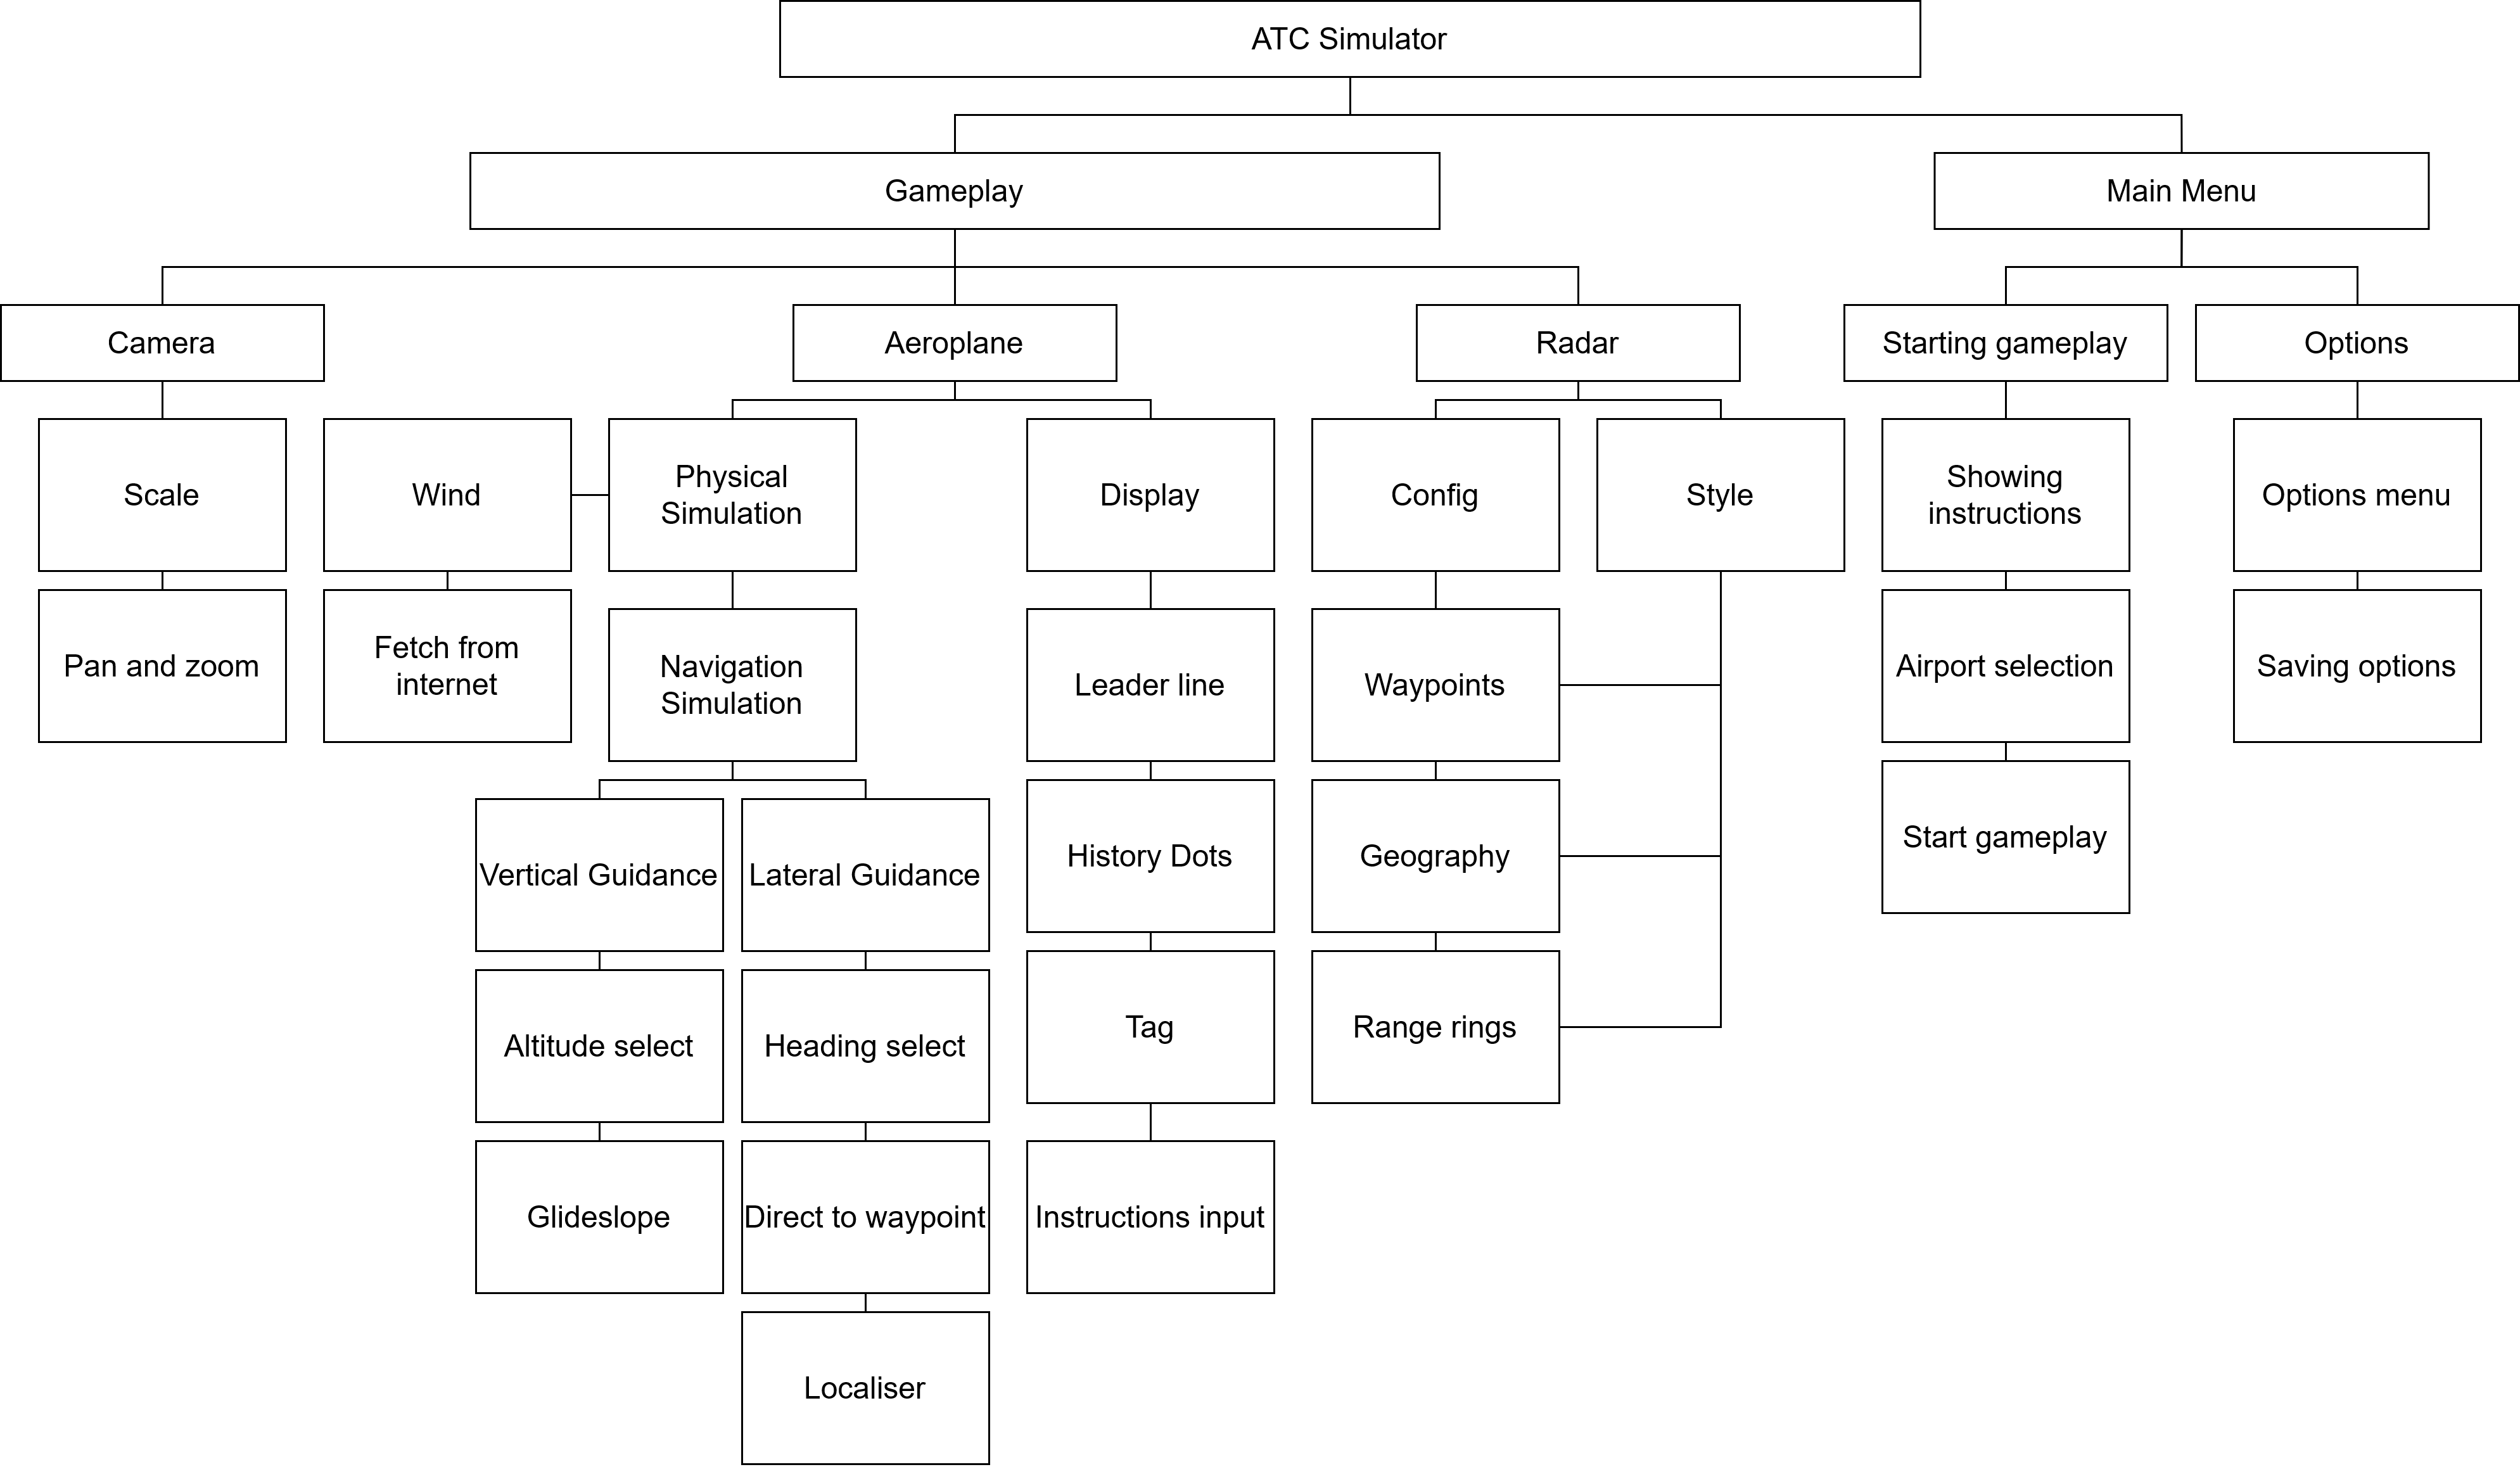
\includegraphics[width=\textwidth]{diagrams/problemdiagram.png}
    \caption{\label{fig:solution_diagram}Solution diagram}
\end{sidewaysfigure}

\clearpage

\section{Design} \label{design}
\subsection{Breakdown of the problem}
Figure \ref{fig:solution_diagram} shows how the problem has been broken down into smaller problems and sub-problems.
Breaking the problem down like this allows each to be solved independently, separating concerns and making development easier because changes to one area do not affect other areas.
The subsequent subsections and their organization will illustrate further the process of choosing how to break down the problem.


\subsection{Representing space}
My simulation will be simulating real-world places: airports and the world around them.
Therefore I cannot use arbitrary units for position or approximate where things are.
Equally, I cannot simulate motion or calculate where points of interest should appear on the screen using latitude and longitude values alone.
Therefore a working value of the lateral and vertical distances in nautical miles from a reference point must be used, which is calculated once using the latitudes and longitudes.
This abstraction removes the curvature of the earth.

\subsubsection{Scale}
That gives everything a position in nautical miles, which then needs to be converted to a number of pixels for it to be displayed.
A scale factor can be calculated by dividing the number of pixels available on the screen by the number of nautical miles that should be shown in that area.
The values in nautical miles can then simply be multiplied by this factor.

\subsubsection{Pan and zoom}
The initial scale can be calculated from a desired width in nautical miles specific to each airport configuration.
From there the user should be able to zoom in or out using the scroll wheel of their mouse.
Each time the user zooms in or out an increment, the scale value will be multiplied by e.g. 1.1 or 0.9 respectively.

Panning the simulated radar screen will be accomplished by recording the position of the user's mouse on the screen when they first press the right mouse button down, and then moving a virtual camera in the inverse direction to the motion of the mouse relative to that point.

\subsection{Simulated aeroplanes}
In order to maintain physical consistency (e.g. if an aeroplane is already in a turn to the right, it will take longer to start turning to the left than if it was not turning), the navigation system will be isolated from the physical simulation and will interact with it by commanding a yaw rate in degrees per second and a \gls{flightpathangle} in degrees.
I have chosen these parameters to provide a level of abstraction which is sufficiently realistic, while keeping complexity reasonably low.

\begin{figure}[H]
\centering
\begin{tabular}{ |l| } 
\hline
\multicolumn{1}{ |c| }{\textbf{Aeroplane}} \\
\hline
TrueAltitude : float \\
TrueAirspeed : float \\
TrueHeading : float \\
PositionNm : Vector2 \\
GroundVector : Vector2 \\
LateralGuidanceMode : LateralMode \\
VerticalGuidanceMode : VerticalMode \\
\hline
void PhysicsUpdate(float) \\
\hline
\end{tabular}
\caption{\label{fig:aeroplaneclass}Aeroplane class diagram}
\end{figure}

Figure \ref{fig:aeroplaneclass} shows the key attributes and methods of the aeroplane class which will be used.
Using a class enables many aeroplanes to be simulated at once, where each aeroplane is an instance of the class.
Keeping track of the many variables of each necessary for the physics and navigation simulation would otherwise be very difficult.

\begin{figure}[H]
\centering
\begin{tabular}{ |c|c|c| }
\hline
Attribute & Units & Valid range \\
\hline
TrueAltitude & Feet & $x \geq 0$ \\
\hline
TrueAirspeed & Knots & $x \geq 0$ \\
\hline
TrueHeading & Degrees & $0 \leq x \leq 360$ \\
\hline
\end{tabular}
\caption{\label{fig:aeroplaneclassinputs}Aeroplane class input validation ranges}
\end{figure}

Figure \ref{fig:aeroplaneclassinputs} shows the valid ranges of the attributes of the Aeroplane class.
Attributes not shown in the table do not require validation because they do not receive user input.
TrueAltitude must be greater than zero because it represents height above terrain and the aeroplane should not go below it; TrueAirspeed cannot be less than zero because it represents forward speed through the air; and TrueHeading, being a heading, is by definition between zero and 360 degrees.
Ensuring that these values remain in a valid range means that all areas of the solution know what to expect and do not each have to do their own validation.

\subsubsection{Physics simulation}
\begin{figure}[H]
\centering
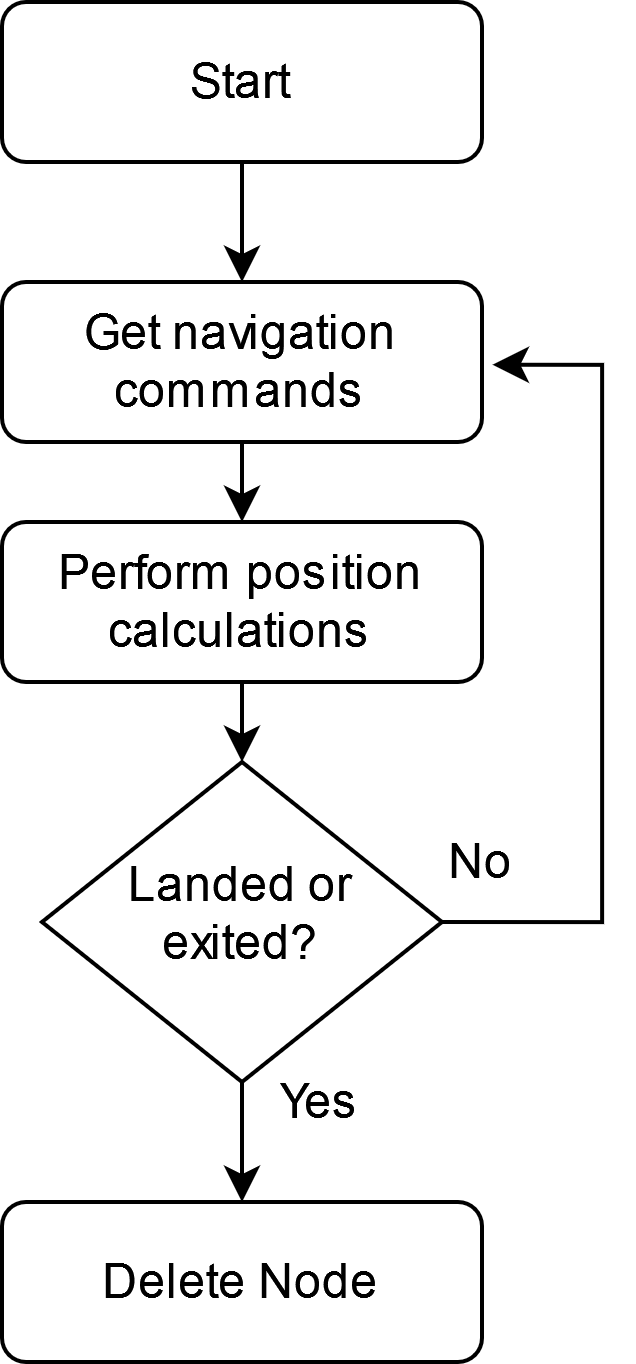
\includegraphics{diagrams/flowcharts/aeroplanesimulationprocess.png}
\caption{\label{fig:physics}Simulation loop}
\end{figure}

As shown in figure \ref{fig:physics}, the aeroplane physics simulation will use a loop in which it will talk to the navigation system to receive its commands for movement, and then update the flight parameters and re-calculate position.
In all calculations the real world time since the last loop iteration will be used to make sure that timescales, e.g. the time it takes for the aircraft to bank left and right, are consistent.
To simulate those times, the flight parameters will be moved towards the commanded values with a rate multiplied by the time delta on each iteration of the loop.
Through testing in a flight simulator I found typical values for those rates: yaw will change at a rate of $\frac{1}{2}$ degrees per second (per second); flight path angle at 0.17 degrees per second (per second); and airspeed at 1 knot per second.
These values will be stored in constant variables.
This loop should run many times a second to provide sufficient accuracy.

To perform the position update, the true heading of the aeroplane will be converted to a \gls{directionvector} which will be multiplied by the true airspeed.
The fact that the ground speed is lower given the same airspeed if the \gls{flightpathangle} deviates from zero will be accounted for.

\subsubsection{Navigation simulation}
At all times, a separate lateral and vertical guidance mode will be engaged.
Making lateral and vertical modes independent of each other reduces code duplication because it is often required to have e.g. the same lateral behaviour with multiple vertical behaviours.
This also mirrors how autopilots work in reality.
Every simulation step, the active modes will be asked if they want to change to a different mode, which will be used for example when maintaining a heading while waiting to capture the localizer.
The modes will each be classes which will inherit from a parent class: LateralMode (figure \ref{fig:lateralmodeclass}) for the lateral modes and VerticalMode (figure \ref{fig:verticalmodeclass}) for the vertical modes, overriding e.g. the RollCommand method to implement their own functionality.
Because the LateralMode and VerticalMode classes have a common attribute of aeroplane, the aeroplane for which they are providing guidance, this will be in a parent class Mode (figure \ref{fig:guidancemodeclass}) which they will inherit from.
Figure \ref{fig:vertnav} and \ref{fig:lnav} illustrate how the vertical and lateral guidance modes respectively of an aeroplane will change on certain conditions.
% The modes will each be classes which will implement \glspl{interface} stating that they include e.g. an update function.

\begin{figure}[H]
\centering
\begin{tabular}{ |l| } 
\hline
\multicolumn{1}{ |c| }{\textbf{Mode}} \\
\hline
aeroplane : Aeroplane \\
\hline
\end{tabular}
\caption{\label{fig:guidancemodeclass}Guidance mode class diagram}
\end{figure}

\begin{figure}[H]
\centering
\begin{tabular}{ |l| } 
\hline
\multicolumn{1}{ |c| }{\textbf{VerticalMode : Mode}} \\
\hline
float FlightPathAngleCommand() \\
VerticalMode? NewMode() \\
\hline
\end{tabular}
\caption{\label{fig:verticalmodeclass}Vertical mode class diagram}
\end{figure}

\begin{figure}[H]
\centering
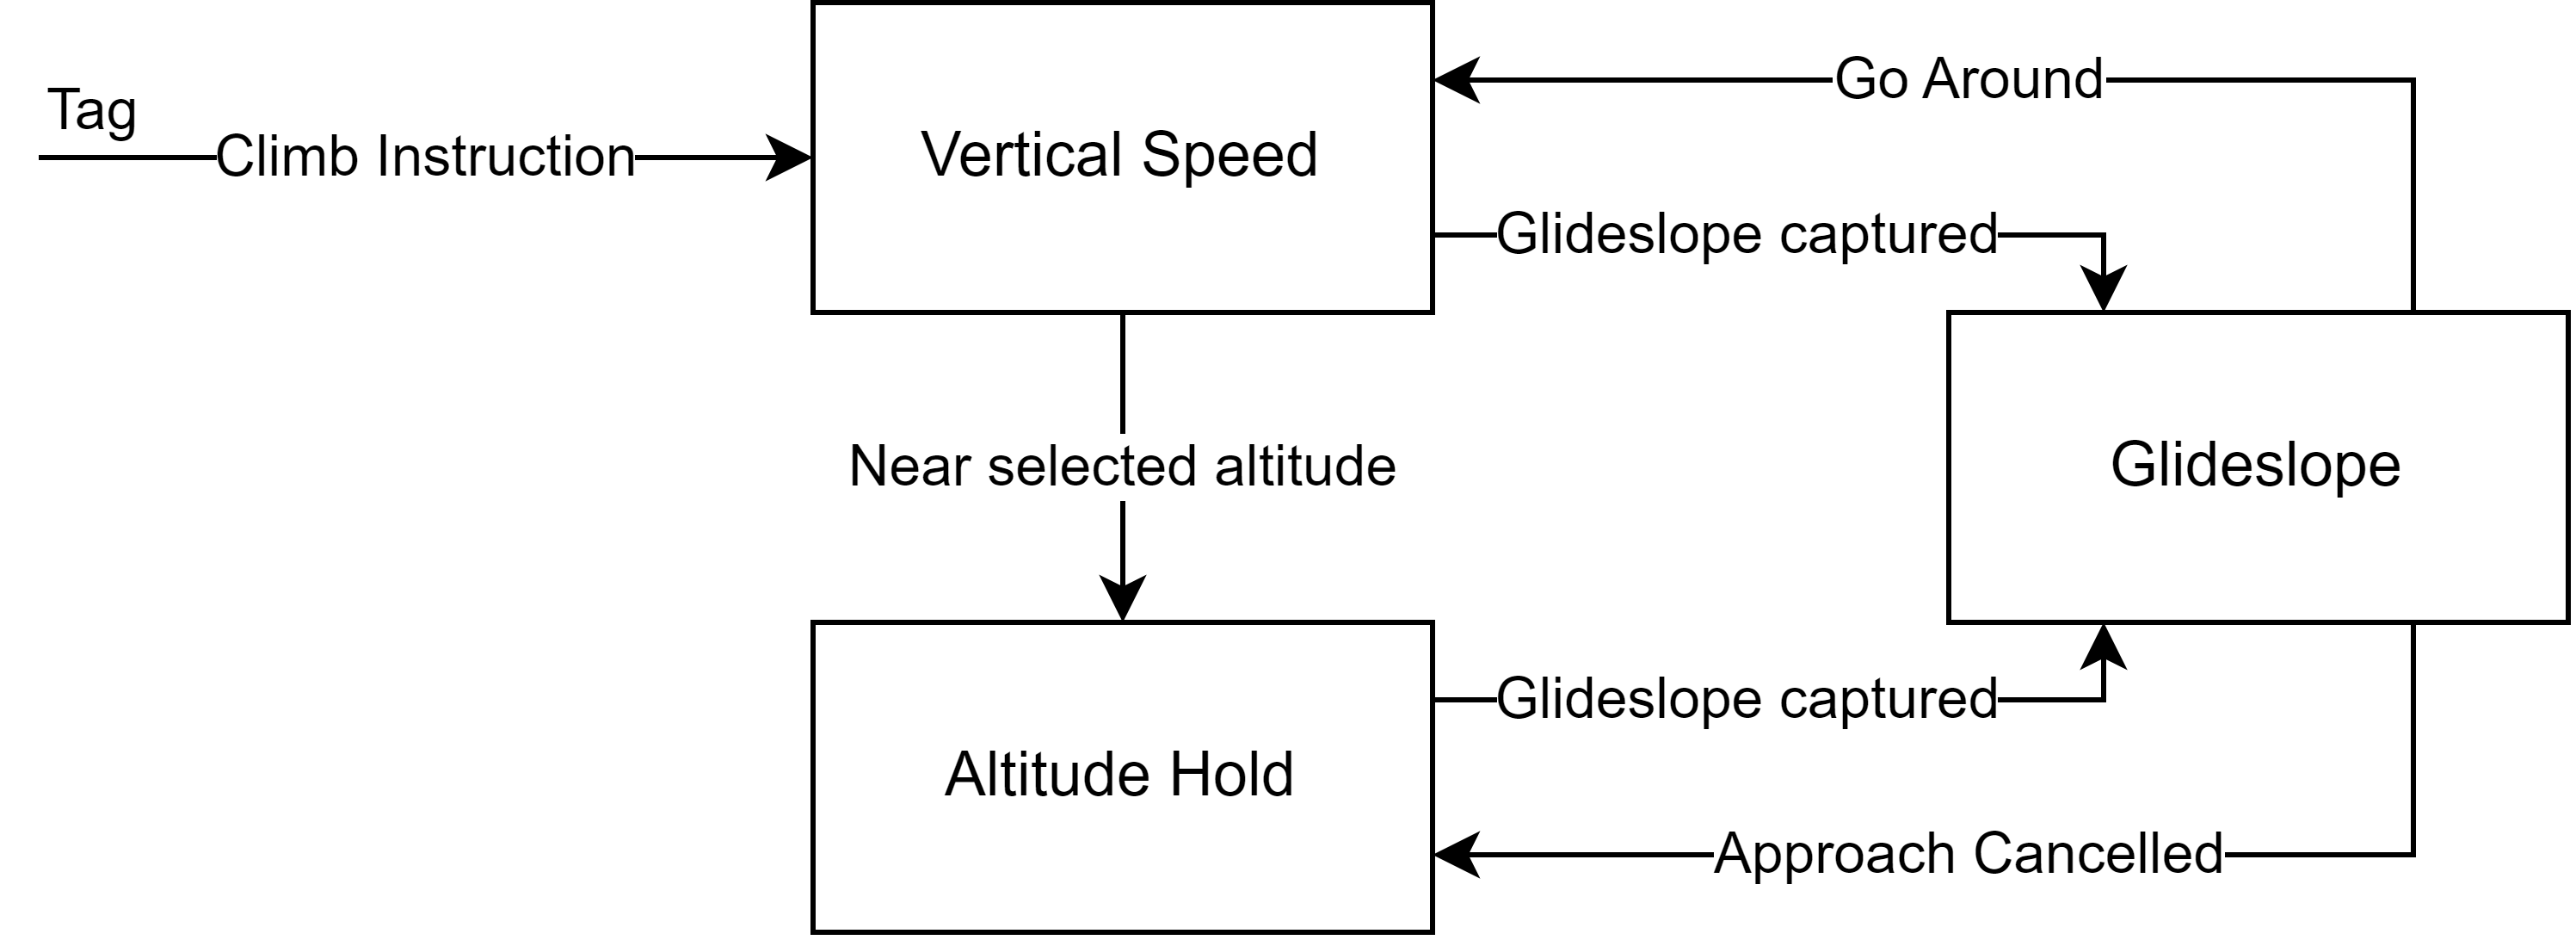
\includegraphics{diagrams/vertnav.png}
\caption{\label{fig:vertnav}State transitions between vertical guidance modes}
\end{figure}

\paragraph{Altitude change modes}
When an instruction to climb or descend is given a vertical guidance mode such as vertical speed will be engaged.
The vertical speed mode will control the commanded flight path angle to achieve the desired vertical speed, and then once the aeroplane is calculated to be close enough to the instructed altitude that if it levels off at the standard rate it will arrive at that altitude without over or undershooting, the mode will tell the guidance system to switch to the altitude hold mode.
Figure \ref{fig:verticalspeedmodeclass} shows the class which will implement the vertical speed mode, overriding the base FlightPathAngleCommand and NewMode methods and adding new attributes.
The class which implements the altitude hold mode does not override the base methods, which are to return zero for the FlightPathAngleCommand and null (i.e. do not change mode) for the NewMode method; it also does not require additional attributes.

\begin{figure}[H]
\centering
\begin{tabular}{ |l| } 
\hline
\multicolumn{1}{ |c| }{\textbf{VerticalSpeed : VerticalMode}} \\
\hline
float Altitude \\
float VerticalRate \\
\hline
float FlightPathAngleCommand() \\
VerticalMode? NewMode() \\
\hline
\end{tabular}
\caption{\label{fig:verticalspeedmodeclass}Vertical speed mode class diagram}
\end{figure}

\paragraph{Glideslope}
When the aeroplane is cleared for an \acrshort{ils} approach, the active vertical guidance mode will wait until the aeroplane approaches an appropriate distance from the glideslope, and then tell the guidance system to switch to the glideslope follow mode which will command a pitch down to match the glideslope angle.
This will require calculating the current height of the glideslope beam at the aeroplane's position based on the position and elevation of the transmitter; and the angle of the glideslope.

\begin{figure}[H]
\centering
\begin{tabular}{ |l| } 
\hline
\multicolumn{1}{ |c| }{\textbf{LateralMode : Mode}} \\
\hline
float RollCommand() \\
LateralMode? NewMode() \\
\hline
\end{tabular}
\caption{\label{fig:lateralmodeclass}Lateral mode class diagram}
\end{figure}

\begin{figure}[H]
\centering
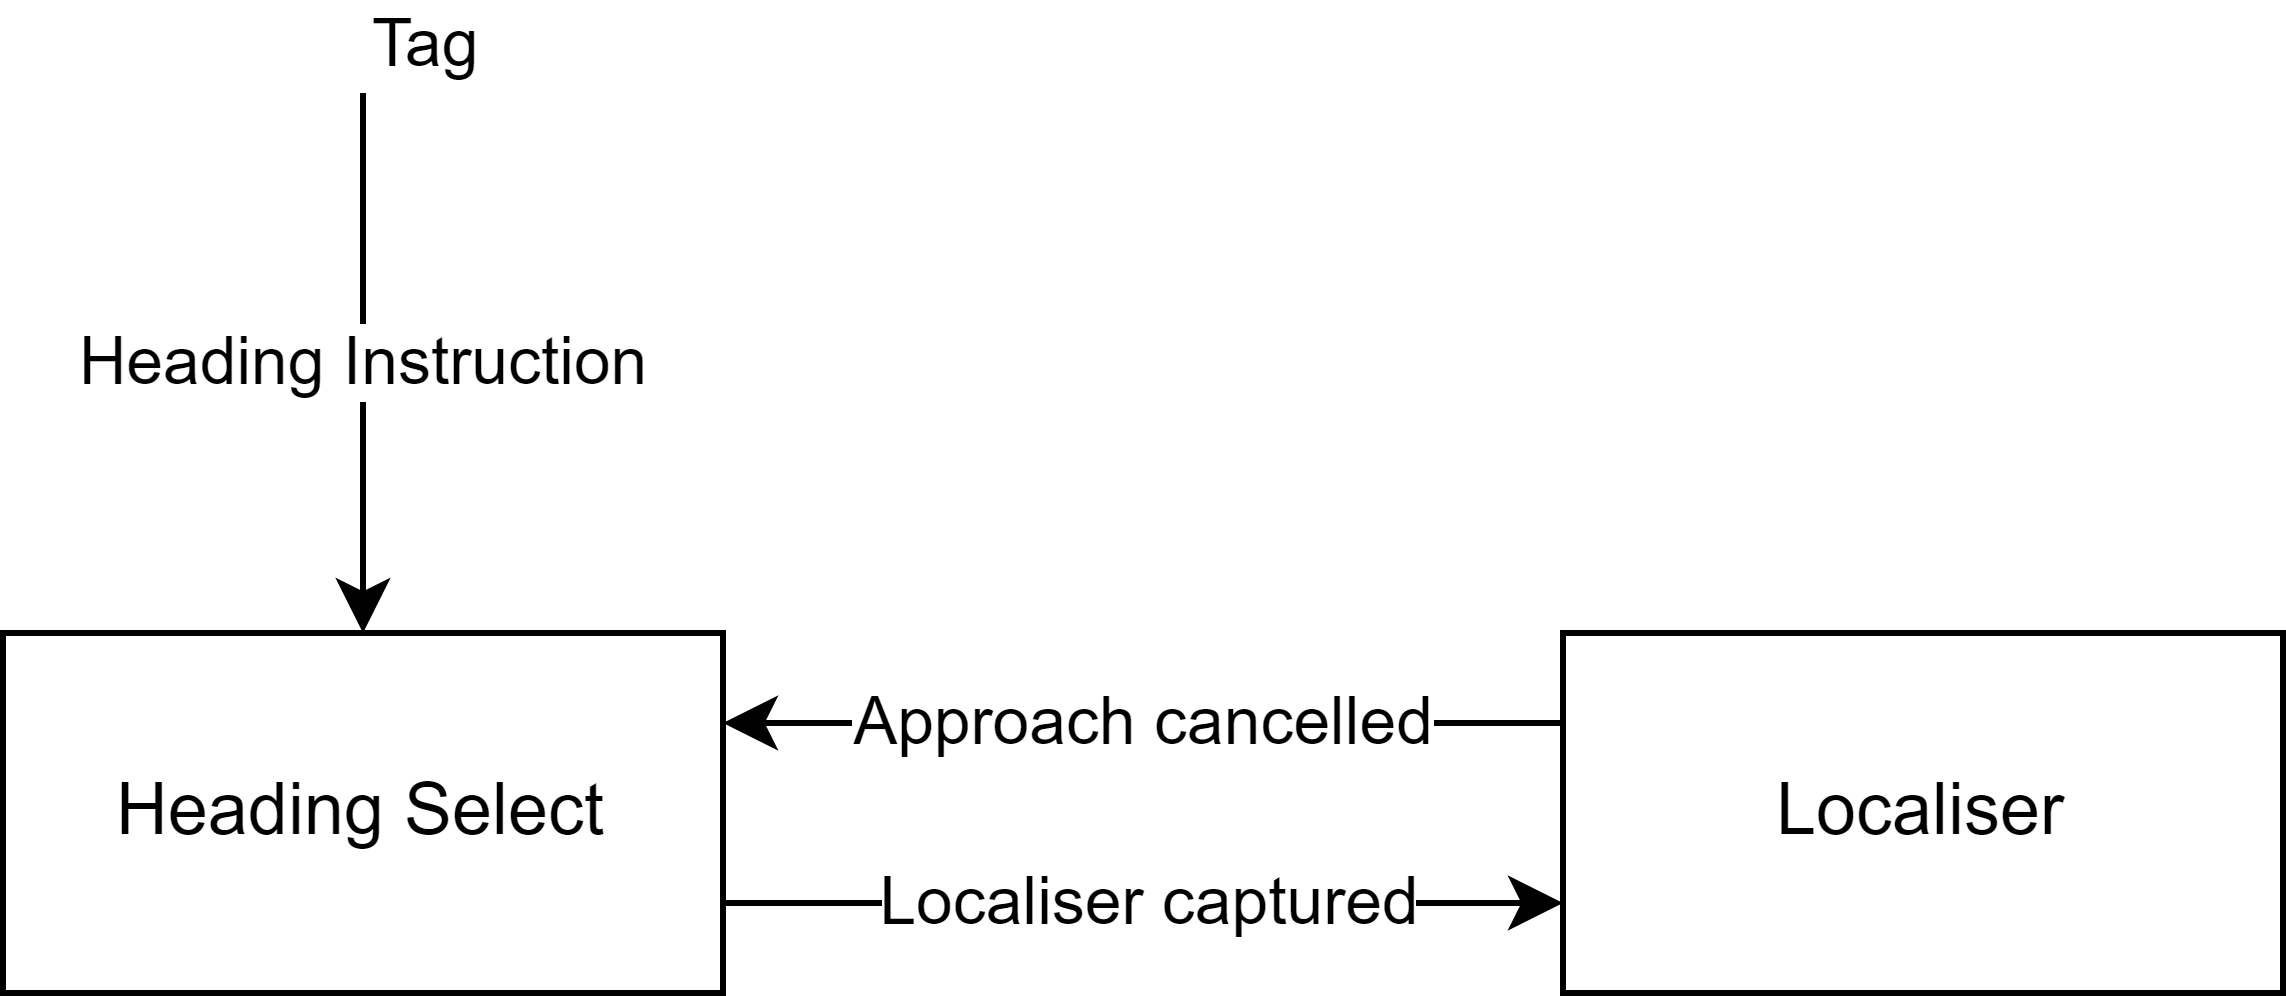
\includegraphics{diagrams/lnav.png}
\caption{\label{fig:lnav}State transitions between lateral modes}
\end{figure}


\subsection{Interface}
Because it is effective in ATC-Sim (section \ref{atc-sim}), the simulator will have two main screens: a main menu where the user can select which airport they want to control at, and a separate gameplay screen they will be taken to where that will take place.
Each will be a separate 'scene' in Godot, which can be created independently.

\subsubsection{Main menu}
\begin{figure}[H]
\centering
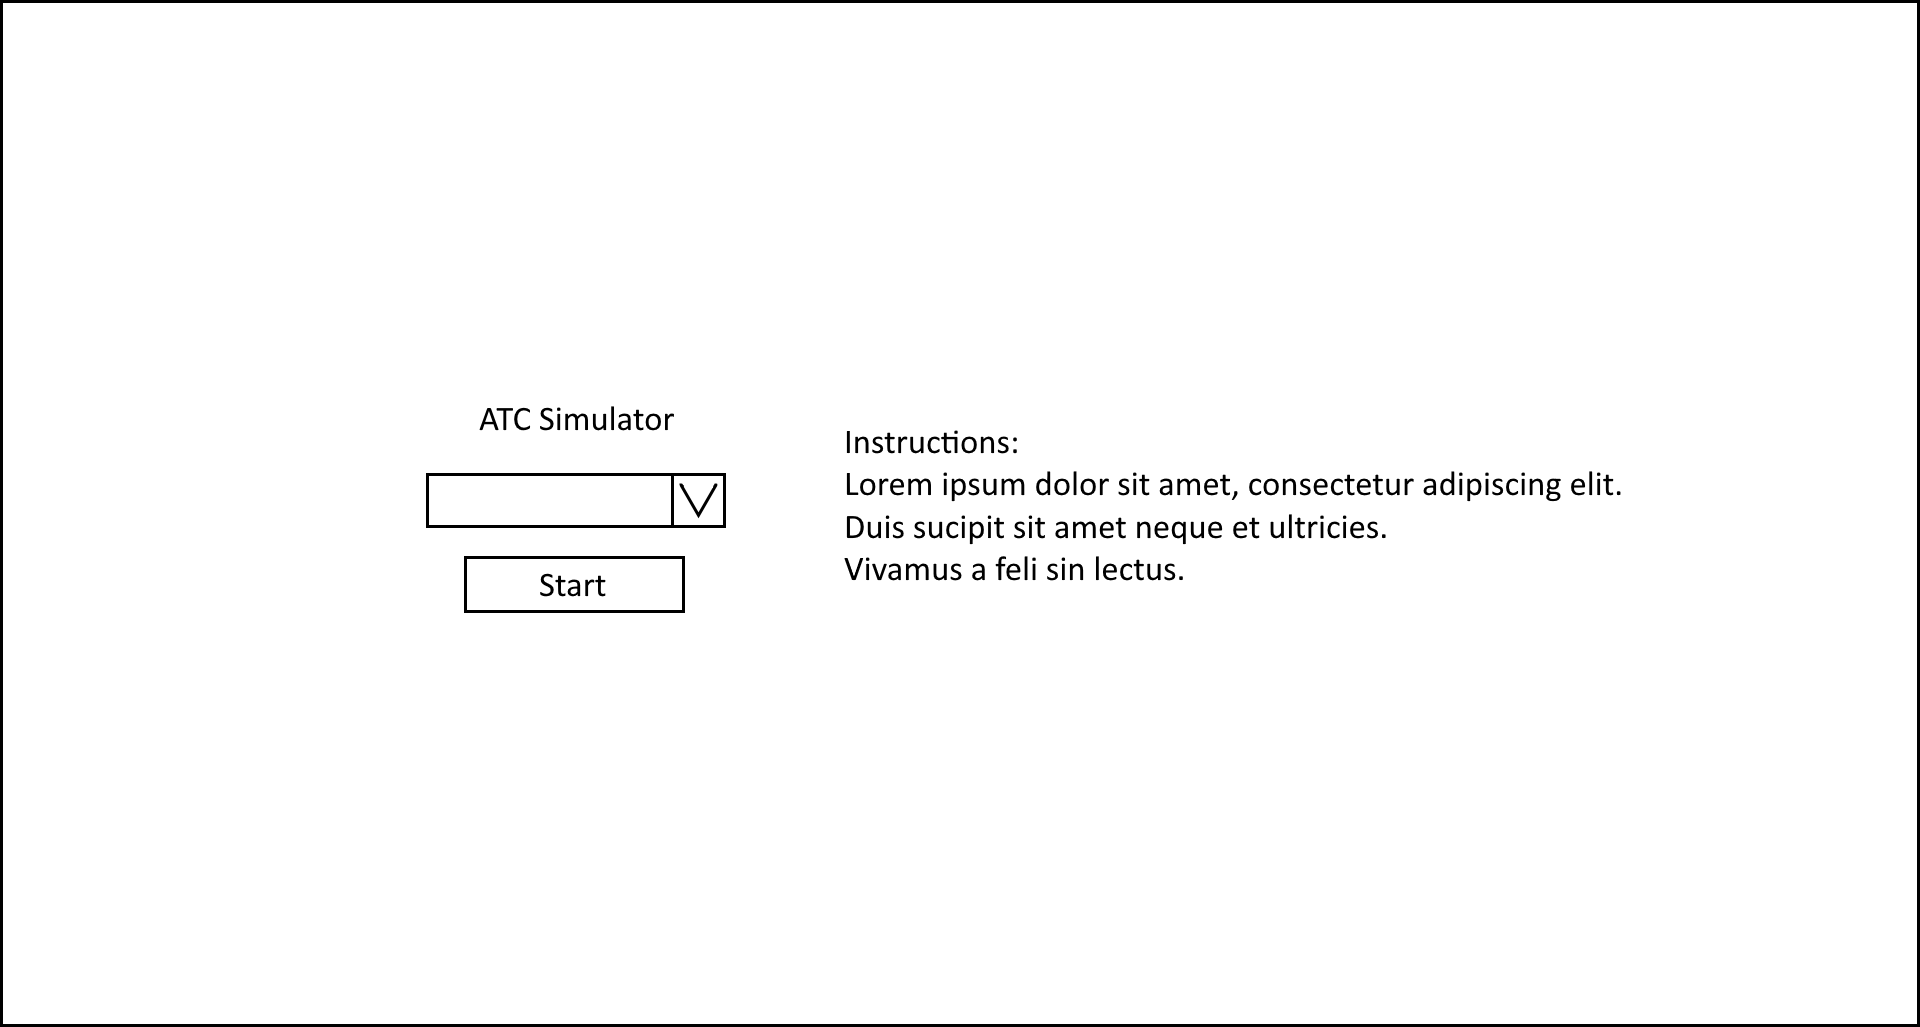
\includegraphics[width=\textwidth]{diagrams/mainmenu.png}
\caption{\label{fig:main_menu_design}Main menu screen design}
\end{figure}

Figure \ref{fig:main_menu_design} shows an approximate and simple design for a main menu.
A dropdown menu will be present which will be populated with the airport options available stored on the computer, with one of them selected by default.
A button directly below it will initiate the gameplay.
This should be fairly intuitive and usable.
Some text can be shown to give some help with how to use the simulation.

\subsubsection{Displaying aeroplanes}
\begin{figure}[H]
\centering
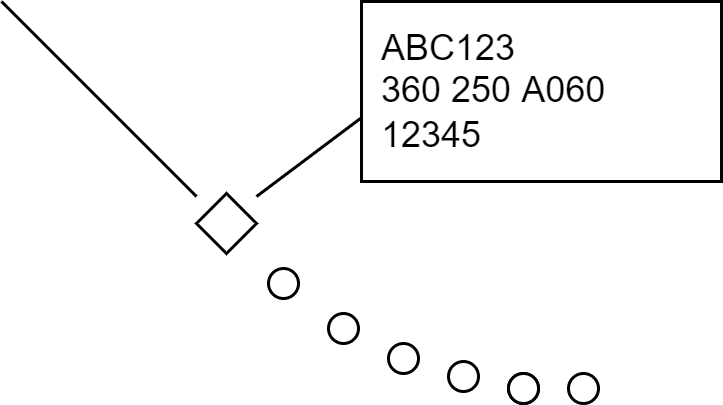
\includegraphics[width=0.5\textwidth]{diagrams/aeroplane_design.png}
\caption{\label{fig:aeroplane_design}Design of the aeroplane display}
\end{figure}

Figure \ref{fig:aeroplane_design} shows the four main features of the aeroplane interface.
\begin{itemize}
    \item The blip: a dot or other symbol showing the last known position of the aeroplane, which the other features are centred around.
    \item The leader line: a line pointing in the last known direction of travel.
    \item History dots: a series of dots or other symbols showing the previously received positions of the aeroplane, illustrating its motion.
    \item The tag: a box which can be dragged around relative to the blip showing information about the aeroplane; it will also be used to give instructions to the aeroplane.
\end{itemize}

\subsubsection{Giving instructions to aeroplanes}
As described in section \ref{existingsolutions}, there are various approaches to this.
One is to use text input.
The problem with this is that, especially for users who are slow at typing, it may be slow to use; also the user could make a typo which would require them to type the instruction out again.
Another approach is to use mouse movements.
This would be faster and more intuitive to use but would compromise on realism and might not enable me to offer the complex set of instructions necessary.
Therefore to strike the best balance between usability and realism, I will use a system in which the user enters values into input boxes on the tags next to the aeroplane, and more complicated options will be presented through drop-down menus on the tag.


\subsection{Waypoints}
\begin{figure}[H]
\centering
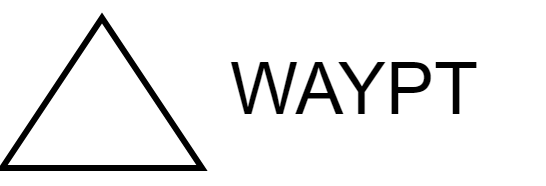
\includegraphics{diagrams/waypointdesign.png}
\caption{\label{fig:waypointdesign}Waypoint design}
\end{figure}

Waypoints should appear on the screen as in the diagram, with a symbol depending on their type and text with their name next to them.


\subsection{Usability features}
TODO


\clearpage
\section{Development}
I have chosen to use the Godot game engine\footnote{\url{https://godotengine.org/}} to build my simulator.
It works using a system of nodes, which I can use to hold each module of my solution.


\subsection{Data}
Many problems of the solution shown require data to be stored.
This includes waypoints, geography, airports, and more.
The Godot game engine provides a feature called \textit{resources}, which are data containers that allow you to define the names and data types of fields that the resource should store; then the engine manages writing this to the disk in an appropriate place as a text file.
This is very convenient because it abstracts away the details of handling files on different operating systems and allows an object-oriented style approach to data storage where fields can contain references to other resource types, for example a RadarConfig resource will contain an array of references to Waypoint resources.
It also provides data types such as vectors.
% \begin{center}
% \begin{tabular}{ | p{5em} | p{20em} | } 
%     \hline
%     Waypoint &
%     \begin{itemize}
%         \item Vector2 LatitudeLongitude
%         \item string Name
%     \end{itemize}
%     \\ 
%     \hline
%     Airport & TODO \\ 
%     \hline
% \end{tabular}
% \end{center}


\subsection{Mapping the real world onto the screen}
Several features of my solution need to work with real-world points, such as \glspl{waypoint}, defined by latitudes and longitudes.
To make these easier to work with, I decided to convert their positions from latitudes and longitudes into Cartesian coordinates, with the screen centre as (0, 0).
To do this, I would need to assign the centre of the screen a latitude and longitude, and then calculate the point's lateral and vertical distances from it.
If I wanted to display the point on the screen, I would then need to scale the real-world distances to pixels.

To enable this I created a class, 'Geo', to provide re-usable geographical functions.
For example whilst the function shown in listing \ref{lst:getdistancenm} was initially created to enable displaying waypoints on the screen, it can also be used to for example display geographical features.

\subsubsection{Calculating distance along the Earth}
I chose to use the spherical law of cosines formula to calculate distance, since with modern floating point numbers, it does not have significant rounding errors for the distances seen in my solution.
It states that where $\phi _{1}, \lambda _{1}$ and $\phi _{2}, \lambda _{2}$ are the latitudes and longitudes of two points, and ${\Delta \phi, \Delta \lambda}$ are their absolute differences, the central angle between them is given by:
\[ \Delta \sigma =\arccos {\bigl (}\sin \phi _{1}\sin \phi _{2}+\cos \phi _{1}\cos \phi _{2}\cos(\Delta \lambda ){\bigr )} \] 
Because the inputs are given in radians, the result is in radians.
The simple sector length formula $L=r\theta$ can then be used to find the distance, where $r$ is the radius of the Earth\cite{greatcircledistance}.
\lstset{style=csharp}
\begin{lstlisting}[label={lst:getdistancenm},caption=Calculating great-circle distance using the spherical law of cosines]
// Average radius of the Earth in nautical miles
private const float EarthRadiusNm = 3438.175f;

public static float GetDistanceNm(float latitude, float longitude, float otherLatitude, float otherLongitude)
{
    float centralAngle = Mathf.Acos(Mathf.Sin(latitude) * Mathf.Sin(otherLatitude) + Mathf.Cos(latitude) * Mathf.Cos(otherLatitude) * Mathf.Cos(Mathf.Abs(longitude - otherLongitude)));
    return EarthRadiusNm * Mathf.DegToRad(centralAngle);
}
\end{lstlisting}

% Insert more detail about testing here
After testing, I found that this broke somehow.
So I used the haversine formula instead:
TODO: add evidence and elaborate
\[ \operatorname{hav}(\theta ) = \operatorname{hav} (\Delta \phi) + \cos(\varphi _{1})\cos (\varphi _{2})\operatorname{hav}(\Delta \lambda) \] 
\[ d = r \operatorname{archav} (h) \]

\begin{lstlisting}[label={lst:getdistancenmhaversine},caption=Calculating great-circle distance using the haversine formula]
// Convert to radians
float lat = Mathf.DegToRad(latitude);
float lon = Mathf.DegToRad(longitude);
float otherLat = Mathf.DegToRad(otherLatitude);
float otherLon = Mathf.DegToRad(otherLongitude);
// Use the haversine formula
float haversineTheta = Haversine(otherLat - lat) + Mathf.Cos(lat) * Mathf.Cos(otherLat) * Haversine(otherLon - lon);
return EarthRadiusNm * Archaversine(haversineTheta);
\end{lstlisting}

\begin{lstlisting}[label={lst:haversine},caption=The haversine functions]
public static float Haversine(float x)
{
  return Mathf.Pow(Mathf.Sin(x / 2f), 2);
}

public static float Archaversine(float x)
{
  return 2f * Mathf.Asin(Mathf.Sqrt(x));
}
\end{lstlisting}

\subsubsection{Calculating position as a Cartesian coordinate}
By using an imaginary point with the latitude of the screen centre and the longitude of the point, I can individually calculate the horizontal and vertical distances.
Because the distance will always be positive, I have to calculate the \gls{quadrant} the point lies in relative to the screen centre and flip the sign accordingly for it to be a coordinate.
\lstset{style=csharp}
\begin{lstlisting}[caption=Calculating the position of a point relative to another]
public static Vector2 RelativePositionNm(Vector2 position, Vector2 relativeTo)
{
    float horizontalComponent = GetDistanceNm(relativeTo.x, relativeTo.y, relativeTo.x, position.y);
    horizontalComponent = position.y < relativeTo.y ? -horizontalComponent : horizontalComponent;
    float verticalComponent = GetDistanceNm(relativeTo.x, position.y, position.x, position.y);
    verticalComponent = position.x < relativeTo.x ? -verticalComponent : verticalComponent;
    return new Vector2(horizontalComponent, verticalComponent);
}
\end{lstlisting}

\subsubsection{Scaling}
Because the size of the game window will change based on the resolution of the user's monitor and if they resize it, the scale factor has to continually change if a fixed real-world distance is to be displayed, which is necessary for my solution.
It may also be useful to be able to fix the distance by either height or width.
Calculating the scale factor given a desired real-world distance to display is a simple matter of dividing the screen size by that distance.
\lstset{style=csharp}
\begin{lstlisting}[caption=Calculating the scale]
public static new float Scale(Rect2 viewportRect)
{
    _viewportRect = viewportRect;
    float zoomValue = Mathf.Pow(1 + ZoomSpeed, Zoom);
    return RadarConfig.FixedBy switch
    {
        RadarConfig.DisplayFixedBy.Width => (viewportRect.Size.x / RadarConfig.WidthNm) * zoomValue,
        RadarConfig.DisplayFixedBy.Height => (viewportRect.Size.y / RadarConfig.HeightNm) * zoomValue,
        RadarConfig.DisplayFixedBy.Compromise => (viewportRect.Size.x / RadarConfig.WidthNm + viewportRect.Size.y / RadarConfig.HeightNm) / 2 * zoomValue,
        _ => throw new NotImplementedException()
    };
}
\end{lstlisting}
The position in nautical miles of a point can then simply be multiplied by this value to get its final screen position.
\begin{lstlisting}[caption=Notifying other modules of a change in scale]
[Signal] public delegate void ScaleChangedEventHandler();

public override void _Process(double delta)
{
    float scale = Scale(_viewportRect);
    if (scale != _previousScale)
    {
        EmitSignal(nameof(ScaleChanged));
    }
    _previousScale = scale;
}
\end{lstlisting}


\subsection{Aeroplane physical simulation}
The heading of an aeroplane describes the direction it is pointing in, which is not necessarily the same as the direction it is travelling in.
In stable flight the main contributor to this discrepancy is wind, see figure \ref{fig:windtriangle}.

\lstset{style=csharp}
\begin{lstlisting}[caption=Wrapping true heading value]
[Export] public float TrueHeading
{
    get => _heading;
    set => _heading = Mathf.Wrap(value, 0, 360);
}
\end{lstlisting}

To calculate a \gls{vector} representing the movement of an aeroplane over the ground the heading \gls{vector} and wind \gls{vector} are added, where the \gls{heading} \gls{vector} is the aeroplane's \gls{directionvector} multiplied by its \gls{airspeed} and the wind \gls{vector} is the wind \gls{directionvector} multiplied by the wind speed.
\lstset{style=csharp}
\begin{lstlisting}[caption=Extract of the aeroplane physics process]
Vector2 airVector = HeadingToVector(TrueHeading) * TrueAirspeed;
Vector2 windVector = HeadingToVector(_simulator.WindDirection) * _simulator.WindSpeed;
Velocity = (airVector + windVector) / SecondsInAnHour * (float)delta;
PositionNm += Velocity;
\end{lstlisting}

\subsubsection{Converting a heading to a direction vector}
To convert a \gls{heading} to a \gls{directionvector} it is necessary to determine which \gls{quadrant} the \gls{heading} lies in.
The angle the \gls{heading} makes with the $y$ axis can then be calculated.
Then the sine rule can be used to calculate the positive $x$ and $y$ components of a \gls{unitvector} with that angle.
Knowing which \gls{quadrant} the \gls{heading} lies in, the sign of the components can be changed appropriately by multiplying each by $1$ or $-1$.
\lstset{style=csharp}
\begin{lstlisting}[caption=Converting a heading to a vector]
private Vector2 HeadingToVector(float heading)
{
  Vector2 quadrant = new Vector2(1, 1);
  float theta = heading;
  if (heading > 270)
  {
    theta = 360 - heading;
    quadrant = new Vector2(-1, 1);
  }
  else if (heading > 180)
  {
    theta = heading - 180;
    quadrant = new Vector2(-1, -1);
  }
  else if (heading > 90)
  {
    theta = 180 - heading;
    quadrant = new Vector2(1, -1);
  }
  return new Vector2(Mathf.Sin(Mathf.DegToRad(theta)), Mathf.Sin(Mathf.DegToRad(90 - theta))) * quadrant;
}
\end{lstlisting}


\subsection{Aeroplane navigation simulation}
\subsubsection{Glideslope}
Because it would be difficult to add the debugging features necessary to the main project, I chose to create a python program which would run a simplified simulation and allow me to more quickly iterate on the glideslope vertical mode parameters and see the result.
I initially chose to use a PID controller\cite{pidcontroller} because it is probably similar to what is done in real life, however it was difficult to get it to perform accurately.
Therefore I chose to use a simpler solution which would, based on the time necessary to pitch down to match the glideslope's angle, calculate the point at which to command pitch down in order to align with the glideslope's path.

TODO: Add evidence


\subsection{Aeroplane display}
TODO: explain aeroplane display system
\begin{figure}[H]
\centering
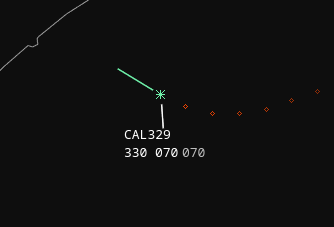
\includegraphics[width=0.75\textwidth]{screenshots/aeroplane.png}
\caption{\label{fig:aeroplane}A screenshot of the game showing the aeroplane display}
\end{figure}

\section{Evaluation}
TODO
\begin{figure}[H]
\centering
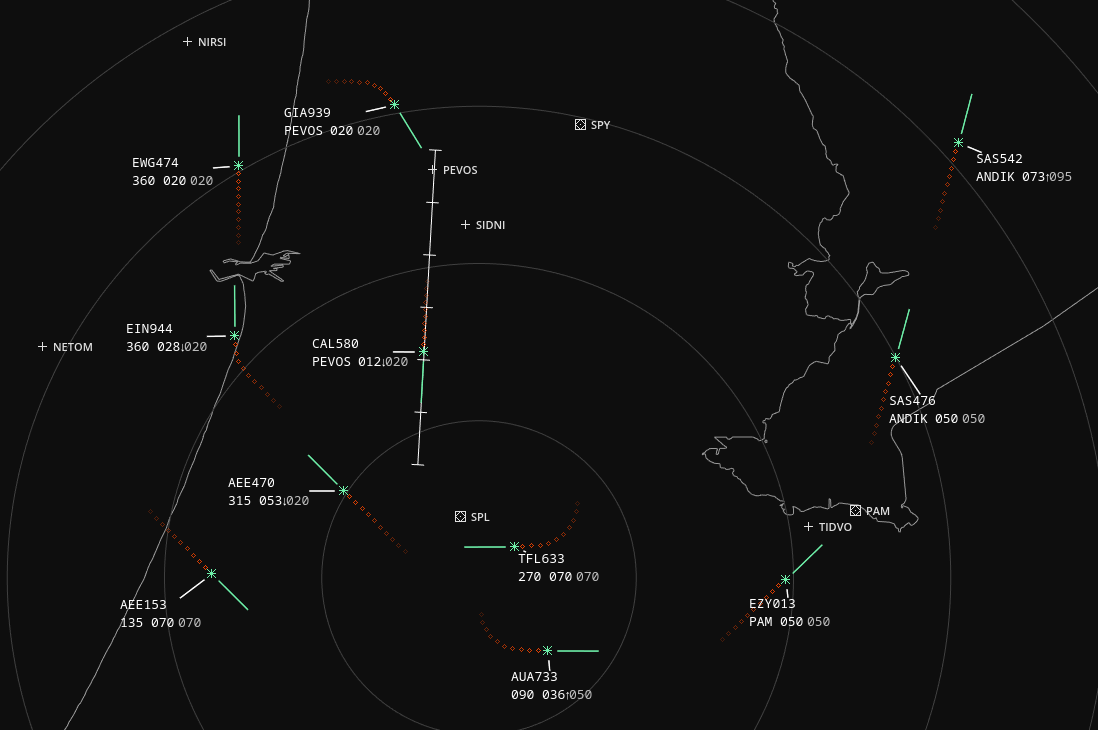
\includegraphics[width=\textwidth]{screenshots/schiphol2.png}
\caption{\label{fig:schiphol}A screenshot of the simulation showing Schiphol airport}
\end{figure}


\subsection{Function and robustness testing}
TODO


\subsection{Usability testing}
TODO


\subsection{Conclusion}
TODO


\clearpage

% References
\printbibliography
\addcontentsline{toc}{section}{References}

% Glossaries
\printnoidxglossaries

% Appendices
\begin{appendices}
\section{Other Code}\label{appendix:otherfunctions}


\section{Other Images}\label{appendix:otherimages}
\begin{figure}[H]
\centering
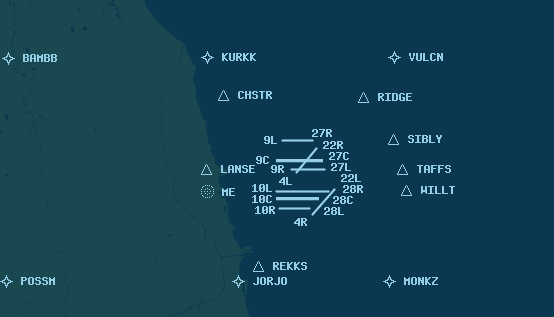
\includegraphics[width=0.75\textwidth]{existing_solutions/airportinseaatcsim.png}
\caption{\label{fig:airportinseaatcsim}Airport appears to be in the sea in ATC-SIM}
\end{figure}
\end{appendices}

\end{document}
